\documentclass[class=cs480,notes,tikz]{agony}
\usetikzlibrary{matrix}
\counterwithout{section}{chapter}
\counterwithin{equation}{section}
\renewcommand{\theequation}{\thesection.\alph{equation}}
\creflabelformat{equation}{#2\textup{#1}#3}

\title{CS 480/680 Winter 2024: Lecture Notes}
\begin{document}
\renewcommand{\contentsname}{CS 480/680 Winter 2024:\\{\huge Lecture Notes}}
\thispagestyle{firstpage}
\tableofcontents

Lecture notes taken, unless otherwise specified,
by myself during section 002 of the Winter 2024 offering of CS 480/680,
taught by Hongyang Zhang and Yaoliang Yu.

\begin{multicols}{2}
  \listoflecture
\end{multicols}

\chapter{Classic Machine Learning}

\section{Introduction}
\lecture{Jan 9}

There have been three historical AI booms:
\begin{enumerate}[1.,nosep]
  \item 1950s--1970s: search-based algorithms (e.g., chess),
        failed when they realized AI is actually a hard problem
  \item 1980s--1990s: expert systems
  \item 2012 -- present: deep learning
\end{enumerate}

Machine learning is the subset of AI where a program can learn from experience.

Major learning paradigms of machine learning:
\begin{itemize}[nosep]
  \item Supervised learning: teacher/human labels answers (e.g., classification, ranking, etc.)
  \item Unsupervised learning: without labels (e.g., clustering, representation, generation, etc.)
  \item Reinforcement learning: rewards given for actions (e.g., gaming, pricing, etc.)
  \item Others: semi-supervised, active learning, etc.
\end{itemize}

Active focuses in machine learning research:
\begin{itemize}[nosep]
  \item Representation: improving the encoding of data into a space
  \item Generalization: improving the use of the model on new distributions
  \item Interpretation: understanding how deep learning actually works
  \item Complexity: improving time/space requirements
  \item Efficiency: reducing the amount of samples required
  \item Privacy: respecting legal/ethical concerns of data sourcing
  \item Robustness: gracefully failing under errors or malicious attack
  \item Applications
\end{itemize}

\lecture{Jan 11}
A machine learning algorithm has three phases:
training, prediction, and evaluation.

\begin{defn}[dataset]
  A \term{dataset} consists of a list of \term[feature]{features}
  $\x_1,\dotsc, \x_n, \x_1', \dotsc, \x_m' \in \R^d$
  which are $d$-dimensional vectors and a label vector $\vb y\trans \in \R^n$.

  Each \term{training sample} $\x_i$ is associated with a \term{label} $y_i$.
  A \term{test sample} $\x'_i$ may or may not be labelled.
\end{defn}

\begin{example}[email filtering]
  Suppose we have a list $D$ of $d$ English words.

  Define the training set $X = [\x_1,\dotsc,\x_n] \in \R^{d\times n}$ and $\vb y = [y_1,\dotsc,y_n] \in \{\pm1\}^n$
  such that $\x_{ij} = 1$ if the word $j \in D$ appears in email $i$
  (this is the \term{bag-of-words representation}):

  \begin{center}
    \begin{tabular}{cCCCCCC|C}
              & \x_1 & \x_2 & \x_3 & \x_4 & \x_5 & \x_6 & \x' \\ \hline
      and     & 1    & 0    & 0    & 1    & 1    & 1    & 1   \\
      viagra  & 1    & 0    & 1    & 0    & 0    & 0    & 1   \\
      the     & 0    & 1    & 1    & 0    & 1    & 1    & 0   \\
      of      & 1    & 1    & 0    & 1    & 0    & 1    & 0   \\
      nigeria & 1    & 0    & 0    & 0    & 1    & 0    & 0   \\ \hline
      $y$     & +    & -    & +    & -    & +    & -    & ?
    \end{tabular}
  \end{center}

  Then, given a new email $\x'_1$, we must determine if it is spam or not.
\end{example}

\begin{example}[OR dataset]
  We want to train the OR function:
  \begin{center}
    \begin{tabular}{cCCCC}
          & \x_1 & \x_2 & \x_3 & \x_4 \\ \hline
          & 0    & 1    & 0    & 1    \\
          & 0    & 0    & 1    & 1    \\ \hline
      $y$ & -    & +    & +    & +
    \end{tabular}
  \end{center}
  This can be represented graphically by finding a line dividing the points:
  \begin{center}
    \begin{tikzpicture}
      \begin{axis}
        \addplot[blue, thick, mark=none] coordinates {(-0.2, 0.8) (0.8, -0.2)};
        \addplot[red, mark=*] coordinates {(0,0)};
        \addplot[ForestGreen, mark=*] coordinates {(0,1)};
        \addplot[ForestGreen, mark=*] coordinates {(1,0)};
        \addplot[ForestGreen, mark=*] coordinates {(1,1)};
      \end{axis}
    \end{tikzpicture}
  \end{center}
\end{example}

\section{Perceptron}\label{ch:p}

\begin{defn}
  The \term{inner product} of vectors $\ip{\vb a}{\vb b}$
  is the sum of the element-wise product $\sum_j a_j b_j$.

  A \term{linear function} is a function $f : \R^d \to \R^d$
  such that for all $\alpha,\beta \in \R$, $\x, \vb z \in \R^d$,
  $f(\alpha\x + \beta\vb z) = \alpha f(\x) + \beta f(\vb z)$.
\end{defn}
\begin{theorem}[linear duality]
  A function is linear if and only if there exists $\w \in \R^d$
  such that $f(\x) = \ip{\x}{\w}$.
\end{theorem}
\begin{prf}
  ($\Rarr$) Suppose $f$ is linear.
  Let $\w := [f(\vb e_1), \dotsc, f(\vb e_d)]$
  where $\vb e_i$ are coordinate vectors. Then:
  \begin{align*}
    f(\x) & = f(x_1\vb e_1 + \dotsb + x_d \vb e_d)     \\
          & = x_1 f(\vb e_1) + \dotsb + x_d f(\vb e_d) \\
          & = \ip{\x}{\w}
  \end{align*}
  by linearity of $f$.

  ($\Larr$) Suppose there exists $\w$ such that $f(\x) = \ip{\x}{\w}$.
  Then: \begin{align*}
    f(\alpha\x + \beta\vb z)
     & = \ip{\alpha\x+\beta\vb z,\w}          \\
     & = \alpha\ip{\x}{\w} + \beta\ip{\x}{\w} \\
     & = \alpha f(\x) + \beta f(\vb z)
  \end{align*}
  since inner products are linear in the first argument.
\end{prf}

\begin{defn}[affine function]
  A function $f(\x)$ where there exist $\w \in \R^d$
  and \term{bias} $b \in \R$ such that $f(\x) = \ip{\x}{\w} + b$.
\end{defn}

\begin{defn}[sign function]
  \[
    \sgn(t) = \begin{cases}
      +1 & t > 0    \\
      -1 & t \leq 0
    \end{cases}
  \]
  It does not matter what $\sgn(0)$ is defined as.
\end{defn}

\begin{defn}[linear classifier]
  $\hat y = \sgn(\ip{\x}{\w} + b)$
\end{defn}

The parameters $\w$ and $b$ will uniquely determine the linear classifier.

\begin{example}[geometric interpretation]
  We can interpret $\hat y > 0$ as a halfspace (see CO 250).
  Then, we can draw something like:
  \begin{center}
    \begin{tikzpicture}
      \begin{axis}[axis lines=middle,
          xlabel=$x_1$,
          ylabel=$x_2$,
          enlargelimits,
          ytick=\empty,
          xtick=\empty,
          xmin=-0.5, xmax=1.5, ymin=-0.5, ymax=1.5,
          samples=60]
        \fill[pattern=north west lines, pattern color=blue!20] (-0.5,1.5) -- (1.5,1.5) -- (1.5,-0.5) -- (0.5,-0.5) -- cycle;
        \addplot[blue, thick, mark=none] coordinates {(-0.5, 1.5) (0.5, -0.5)};
        \addplot[red, mark=*] coordinates {(0,0)};
        \addplot[ForestGreen, mark=*] coordinates {(0,1)};
        \addplot[ForestGreen, mark=*] coordinates {(1,0)};
        \addplot[ForestGreen, mark=*] coordinates {(1,1)};
        \draw[line width=2pt,blue,-stealth](0,0)--(0.75,0.5) node[anchor=south west]{$\w$};
      \end{axis}
    \end{tikzpicture}
  \end{center}
\end{example}

\begin{prop}
  The vector $\w$ is orthogonal to the decision boundary $H$.
\end{prop}
\begin{prf}
  Let $\x, \x' \in H$ be vectors on the boundary $H = \{x : \ip{\w}{\x} + b = 0\}$.
  Then, we must show $\x' - \x = \overrightarrow{\vb{xx'}} \perp \w$.

  We can calculate $\ip{\w}{\x' - \x}
    = \ip{\w}{\x} - \ip{\w}{\x'}
    = -b - (-b) = 0$.
\end{prf}

Originally, the inventor of the perceptron thought it could do anything.
He was (obviously) wrong.

\begin{algorithm}[H]
  \caption{Training Perceptron}
  \begin{algorithmic}
    \Require Dataset $(\x_i, \y_i) \in \R^d \times \{\pm 1\}$,
    initialization $\w_0 \in \R^d$, $b_0 \in \R$.
    \Ensure $\w$ and $b$ for linear classifier $\sgn(\ip{\x}{\w} + b)$
    \For{$t=1,2,\dotsc$}
      \State receive index $I_t \in \{1,\dotsc,n\}$
      \If{$\y_{I_t}\qty(\ip{\x_{I_t}}{\w} + b) \leq 0$}
        \State $\w \gets \w + \y_{I_t}\x_{I_t}$
        \State $b \gets b + \y_{I_t}$
      \EndIf
    \EndFor
  \end{algorithmic}
\end{algorithm}

In a perceptron, we train by adjusting $\w$ and $b$
whenever a training data feature is classified ``wrong''
(i.e., $\vv{score}_{\w,b}(\x) := \y\hat y < 0 \iff$ the signs disagree).

The perceptron solves the feasibility problem
\begin{center}
  Find $\w \in \R^d$, $b \in \R$ such that $\forall i, \y_i(\ip{\x_i}{\w} + b) > 0$
\end{center}
by iterating one-by-one.
It will converge ``faster'' (with fewer $t$-iterations) if the data is ``easy''.

Consider what happens when there is a ``wrong'' classification.
Let $\w_{k+1} = w_k + \y\x$ and $b_{k+1} = b_k + \y$.
Then, the updated score is:
\begin{align*}
  \vv{score}_{\w_{k+1},b_{k+1}}(\x)
   & = \y \cdot (\ip{\x}{\w_{k+1}} + b_{k+1})                                                              \\
   & = \y \cdot (\ip{\x}{\w_k + \y\x} + b_k + \y)                                                          \\
   & = \y \cdot (\ip{\x}{\w_k} + b_k) + \ip{\x}{\x} + 1                                                    \\
   & = \y \cdot (\ip{\x}{\w_k} + b_k) + \underbrace{\norm{\x}_2^2 + 1}_{\mathclap{\text{always positive}}}
\end{align*}
which is always an increase over the previous ``wrong'' score.

\textrule{$\downarrow$ Lectures 3 and 4 taken slides and Neysa since I was sick $\downarrow$}
\lecture{Jan 16}

Instead of writing the affine function $\ip{\x}{\w} + b$,
write $\ip{\x}{\w} = \ip{\mqty(\x\\1)}{\mqty(\w\\b)}$.

Then, the update rule becomes $\w \gets \w + \y\x$.

\begin{theorem}[convergence theorem]
  Suppose there exists $\w^*$ such that $\y_i\ip{\x_i,\w^*} > 0$ for all $i$.
  Assume that $\norm{\x_i}_2 \leq C$ for all $i$, and we normalize the $\w^*$
  such that $\norm{\w^*}_2 = 1$.
  Define the margin $\gamma := \min_i\abs{\ip{\x_i}{\w^*}}$.

  Then, the perceptron algorithm converges after $C^2/\gamma^2$ mistakes.
\end{theorem}
\begin{prf}
  Recall the update on the mistake $(\x,\y)$ is $\w \gets \w + \y\x$.

  Then, the inner product $\ip{\w}{\w^*}$ is
  \begin{align*}
    \ip{\w+\y\x}{\w^*} & = \ip{\w}{\w^*} + \y\ip{\x}{\w^*}     \\
                       & = \ip{\w}{\w^*} + \abs{\ip{\x}{\w^*}} \\
                       & \geq \ip{\w}{\w^*} + \gamma
  \end{align*}
  because $\y\ip{\x}{\w^*}$ must be positive if $\w^*$ is optimal.
  So for each update, $\ip{\w}{\w^*}$ grows by at least $\gamma > 0$.
  That is, after $M$ updates, $\ip{\w}{\w^*} \geq M\gamma$.

  Likewise, the inner product $\ip{\w}$ is
  \begin{align*}
    \ip{\w+\y\x} & = \ip{\w}
    + \underbrace{2\y\ip{\w}{\x}}_{\mathclap{\text{$<0$ because an update means it's wrong}}}
    + \overbrace{\y^2\ip{\w}}^{\mathclap{\text{$\in [0,C^2]$ by construction}}} \\
                 & \leq \ip{\w} + C^2
  \end{align*}
  so each update grows $\ip{\w}$ by at most $C^2$,
  meaning that after $M$ updates, $\ip{\w} \leq MC^2$.

  Finally, recall from linear algebra that
  $1 \geq \cos(\w,\w^*) = \frac{\ip{\w}{\w^*}}{\norm{\w}_2\norm{\w^*}_2}$.
  Then,
  \begin{align*}
    1 & \geq \frac{\ip{\w}{\w^*}}{\norm{\w}_2 \cdot \norm{\w^*}_2} \\
      & \geq \frac{M\gamma}{\sqrt{MC^2} \cdot 1}                   \\
      & = \sqrt{M}\frac{\gamma}{C}
  \end{align*}
  which implies $M \leq C^2/\gamma^2$.
\end{prf}

Therefore, the larger the margin $\gamma$ is, the more linearly separable the data is,
and the faster the perceptron algorithm will converge.

\paragraph{Optimization perspective}
We can equivalently characterize the perceptron algorithm as an optimization problem.
Given the linear classifier $\hat y = \sgn(\ip{\w}{\x})$,
we want to minimize the perceptron loss
\begin{align*}
  \ell(\w,\x_t,\y_t) & = -\y_t\ip{\w}{\x_t} \cdot \I[\text{mistake on $\x_t$}]                            \\
                     & = -\min\{\y_t\ip{\w}{\x_t},0\}                                                     \\
  L(\w)              & = -\frac1n \sum_{t=1}^n \qty(\y_t\ip{\w}{\x_t} \cdot \I[\text{mistake on $\x_t$}])
\end{align*}
Then, the gradient descent update (see \cref{ch:gd}) is
\begin{align*}
  \w_{t+1} & = \w_t - \eta_t \nabla_{\w} \ell(\w_t,\x_t,\y_t)             \\
           & = \w_t + \eta_t \y_t \x_t \cdot \I[\text{mistake on $\x_t$}]
\end{align*}
With step size $\eta_t = 1$, we recover the update rule $\w_{t+1} = \w_t + \y_t\x_t$.

\begin{remark}
  The solution to perceptron is not unique,
  since there are many possible lines separating the data.
\end{remark}

To pick the ``best'' line, we can maximize the margin $\gamma$.
This leads to support vector machines (see \cref{ch:hsvm,ch:ssvm}).

\begin{example}[XOR dataset]\label{exa:xor}
  Consider the XOR function
  \begin{center}
    \begin{tabular}{cCCCC}
           & \x_1 & \x_2 & \x_3 & \x_4 \\ \hline
           & 0    & 1    & 0    & 1    \\
           & 0    & 0    & 1    & 1    \\ \hline
      $\y$ & -    & +    & +    & +
    \end{tabular}
  \end{center}
  There is no separating hyperplane.
\end{example}
\begin{prf}
  Suppose there exist $\w$ and $b$ such that $\y(\ip{\x}{\w} + b) > 0$.
  Then,
  \begin{align*}
    x_1 = (0,0),\y_1 = {-} & \implies b < 0                                   \\
    x_2 = (1,0),\y_2 = {+} & \implies w_1 + b > 0                             \\
    x_3 = (0,1),\y_3 = {+} & \implies w_1 + b > 0 \implies w_1 + w_2 + 2b > 0 \\
    x_4 = (1,1),\y_4 = {-} & \implies w_1 + w_2 + b < 0 \implies b > 0
  \end{align*}
  which is a contradiction.
\end{prf}

This leads us to a theorem.

\begin{theorem}\label{thm:perceptron-fail}
  If there is no perfect separating hyperplane, then the perceptron algorithm cycles.
\end{theorem}

The proof is really complicated, and we will not cover it.

In this case, we can allow some wrong answers by setting a reasonable
loss $\ell$ and regularizer $\operatorname{reg}$:
\[ \min_{\w} \hat{\E}[\ell(\y\hat y) + \operatorname{reg}(\w)] \qq{s.t.} \hat y := \ip{\x}{\w} + b \]

We stop running perceptron when either:
\begin{itemize}[nosep]
  \item the maximum number of iterations is reached (i.e., we keep a constant $\vv{maxiter}$),
  \item the maximum allowed runtime is reached,
  \item the training error stops changing, or
  \item the validation error stops decreasing.
\end{itemize}

If we have multiple classes ($c$ of them),
we can run perceptron as either one-vs.-all or one-vs.-one.

In \term{one-vs.-all perceptron}, for each class $k$,
let it be positive, and all others be negative.
We train weights $\vb w_k$ to get $c$ imbalanced perceptrons.
Then, predict according to the highest score
\[ \hat\y := \argmax_k \ip{\x}{\w_k}. \]

In \term{one-vs.-one perceptron}, for each pair of classes $(k,l)$,
let $k$ be positive, $l$ be negative, and ignore all other classes.
Then, train weights $\w_{k,l}$ for a total of $\binom{c}{2}$ balanced perceptrons.
We predict by majority vote
\[ \hat\y := \argmax_k \sum_{l:l\neq k} \ip{\x}{\w_{k,l}}. \]

\section{Linear Regression}

\lecture{Jan 18}

\begin{problem}[regression]
  Given training data $(\x_i,\y_i) \in \R^{d+t}$, find $f : \mathcal X \to \mathcal Y$
  such that $f(\x_i) \approx \y_i$.
\end{problem}

The problem is that for finite training data,
there are an infinite number of functions that exactly hit each point.

\begin{theorem}[exact interpolation is always possible]
  For any finite training data $(\x_i,\y_i) : {i=1,\dotsc,n}$
  such that $\x_i \neq \x_j$ for all $i \neq j$,
  there exist infinitely many functions $f : \R^d \to \R^t$ such that for all $i$,
  $f(\x_i) = \y_i$.
\end{theorem}


TODO: ...up to slide 14 (geometry of linear regression)

\textrule{$\uparrow$ Lectures 3 and 4 taken from slides and Neysa since I was sick $\uparrow$}

\lecture{Jan 23}

\begin{theorem}[Fermat's necessary condition for optimality]
  If $\w$ is a minimizer/maximizer of a differentiable function $f$
  over an open set, then $f'(\w) = \0$.
\end{theorem}

We can use this property to solve linear regression.

Recall the loss is $\Loss(\W) = \frac1n\norm{\W\X-\Y}^2_F$.
Then, the derivative $\nabla_{\W}\Loss(\W) = \frac2n(\W\X-\Y)\X\trans$.

We can derive the \term{normal equation}:
\begin{align*}
  \frac2n(\W\X-\Y)\X\trans & = 0                           \\
  \W\X\X\trans-\Y\X\trans  & = 0                           \\
  \Aboxed{\W\X\X\trans     & = \Y\X\trans}                 \\
  \W                       & = \Y\X\trans(\X\X\trans)^{-1}
\end{align*}

Once we find $\W$, we can predict on unseen data $\X_{test}$ with $\hat{\Y}_{test} = \W\X_{test}$.

Then,

Suppose $\X = \mqty[0&\epsilon\\1&1]$ and $\vv{y} = \mqty[1&-1]$.

Then, solving the linear least squares regression we get
$\vb{w} = \vv{y}\X\trans(\X\X\trans)^{-1} = \mqty[-2/\epsilon & 1]$.
This is chaotic!

Why does this happen? As $\epsilon\to0$, two columns in $\X$ become almost linearly dependent
with incongruent corresponding $y$-values.
This leads to a contradiction and an unstable $\vb{w}$.

To solve this, we add a $\lambda\norm{\W}_F^2$ term.

\begin{defn}[ridge regression]
  Take the linear regression and add a \term{regularization term}:
  \[ \min_{\W} \frac1n\norm{\W\X-\Y}^2_F + \lambda\norm{\W}^2_F \]
\end{defn}

This gives a new normal equation:
\begin{align*}
  \Loss(\W)                           & = \frac1n\norm{\W\X-\Y}^2_F + \lambda\norm{\W}^2_F \\
  \nabla_{\W}\Loss(\W)                & = \frac2n(\W\X-\Y)\X\trans + 2\lambda\W            \\
  0                                   & = \frac2n(\W\X-\Y)\X\trans + 2\lambda\W            \\
  \Aboxed{\W(\X\X\trans + n\lambda I) & = \Y\X\trans}                                      \\
  \W                                  & = \Y\X\trans(\X\X\trans + n\lambda I)^{-1}
\end{align*}

\begin{prop}
  $\X\X\trans + n\lambda I$ is far from rank-deficient for large $\lambda$.
\end{prop}
\begin{prf}
  Recall from linear algebra that we can always take the singular value decomposition
  of any matrix $M = U\Sigma V\trans$ where $U$ and $V$ are orthogonal
  and $\Sigma$ is non-negative diagonal where the rank is the number of non-zero
  entries in $\Sigma$.

  Consider the SVD of $\X$:
  \begin{align*}
    \X                      & = U\Sigma V\trans                                           \\
    \X\X\trans              & = U\Sigma V\trans V \Sigma\trans U\trans = U\Sigma^2U\trans \\
    \X\X\trans + n\lambda I & = U\Sigma^2U\trans + U(n\lambda I)U\trans                   \\
                            & = U(\Sigma^2 + n\lambda I)U\trans
  \end{align*}
  The matrix $\Sigma^2 + n\lambda I$ is a diagonal matrix with
  strictly positive elements for sufficiently large $\lambda$.
  Therefore, $\X\X\trans + n\lambda I$ has full rank and thus no singular values.
\end{prf}

\begin{remark}
  Performing a ridge regularization is identical to augmenting the data.
\end{remark}

Notice that
\[
  \frac1n\norm{\W\X-\Y}^2_F + \lambda\norm{\W}^2_F
  = \frac1n\norm{\W\mqty[\X & \sqrt{n\lambda}I] - \mqty[\Y & \0]}^2_F
\]
so if we augment $\X$ with $\sqrt{n\lambda}I$ and $\Y$ with $\0$, i.e.,
$p$ data points $\x_j = \sqrt{n\lambda}\e_j$ and $\y_j = 0$.

\section{Logistic Regression}\label{ch:lr}

Return to the linear classification problem.

Recall that we took $\hat{\y} = \sgn(\ip{\x}{\w})$
where $\x = \mqty(\x\\1)$ and $\w = \mqty(\w\\b)$ in $\R^{d+1}$.

How confident are we in our prediction $\hat\y$?
We can use the \term{margin} (or \term{logit}) $\abs{\ip{\x}{\w}}$
(``how far away is the point from the decision boundary?'').

The margin is unnormalized with respect to the data,
so we cannot really interpret it until we somehow cram it into $[0,1]$.

We can try directly learning hte confidence.

Let $\mathcal Y = \{0,1\}$.
Consider confidence $p(\x;\w) := \Pr[\Y = 1 \mid \vv X = \x]$.
Given independent $(\x_i,\y_i)$:
\begin{align*}
    & \Pr[\Y_1 = \y_1,\dotsc,\Y_n=\y_n \mid \vv X_1 = \x_1,\dotsc,\vv X_n = \x_n] \\
  = & \prod_{i=1}^n \Pr[\Y_i = \y_i \mid \vv X_i = \x_i]                          \\
  = & \prod_{i=1}^n [p(\x_i;\w)]^{\y_i}[1-p(\x_i;\w)]^{1-\y_i}
\end{align*}
and we can get our maximum likelihood estimation
\begin{defn}[maximum likelihood estimation]
  \[\max_{\w}\prod_{i=1}^n [p(\x_i;\w)]^{\y_i}[1-p(\x_i;\w)]^{1-\y_i} \]
  or equivalently the minimum minus log-likelihood
  \[ \min_{\w}\sum_{i=1}^n\qty[-\y_i\log p(\x_i;\w)-(1-\y_i)\log(1-p(\x_i;\w))] \]
\end{defn}
Now, how do we define the probability $p$ based on $\w$?

We will assume that the log of the odds ratio $\log\frac{\text{probability of event}}{\text{probability of no event}}
  = \log\frac{p(\x;\w)}{1-p(\x;\w)} = \ip{\x}{\w}$ is linear.

This leads us to the sigmoid transformation.
\begin{defn}[sigmoid transformation]
  \[p(\x;\w) = \frac{1}{1+\exp(-\ip{\x}{\w})}\]
\end{defn}

If we return now to the MLE we defined earlier, we get
\begin{align*}
    & \min_{\w}\sum_{i=1}^n\qty[-\y_i\log p(\x_i;\w)-(1-\y_i)\log(1-p(\x_i;\w))]                                                   \\
  = & \min_{\w}\sum_{i=1}^n\qty[-\y_i\log \frac{1}{1+\exp(-\ip{\x}{\w})} -(1-\y_i)\frac{\exp{-\ip{\x}{\w}}}{1+\exp(-\ip{\x}{\w})}] \\
  = & \min_{\w}\sum_{i=1}^n\qty[\y_i\log(1+\exp(-\ip{\x}{\w}))+(1-\y_i)\log(1+\exp(-\ip{\x}{\w})) + (1-\y_i)\ip{\x}{\w}]           \\
  = & \min_{\w}\sum_{i=1}^n \log[1+\exp(-\ip{\x_i}{\w})] + (1-\y_i)(\ip{\x_i}{\w})
\end{align*}
If we redefine $\y'_i = \frac{\y_i+1}{2}$, i.e., $\y' \in \{\pm1\}$,
then we get the \term{logistic loss}
\begin{equation}\label{eq:lgr}
  \min_{\w} \sum_{i=1}^n \log[1+\exp(-\y'_i\ip{\x}{\w})]
\end{equation}
There is no closed form solution for this problem,
so we use the gradient descent algorithm (covered in \cref{ch:gd}).

Suppose we have found an optimal $\w$.
Then, we can set $\hat y = 1 \iff p(\x;\w) = \Pr[\Y=1\mid\vv X=\x] > \frac12$.
The value of $p(\x;\w)$ is our confidence.

Remember: All this is under the assumption that the log of the odds ratio is linear.
Everything is meaningless if it is not.

\paragraph{Extending to the multiclass case}
Suppose we instead have $\y \in \{1,\dotsc,c\}$ and we need to learn $\w_i$ for each class.
The sigmoid function becomes the \term{softmax} function
\begin{equation}\label{eq:softmax}
  \Pr[\Y = k \mid \vv X = \x; \W = [\w_1,\dotsc,\w_c]]
  = \frac{\exp\ip{\x}{\w_k}}{\sum_{l=1}^c\exp\ip{\x}{\w_l}}
\end{equation}
This maps the real-valued vector $\x$ to a probability vector.
Notice that the softmax values for each class are all non-negative and sum to 1.

To train, we use the MLE again

To predict, pick the index of the highest softmax value
\[ \hat{\y} = \argmax_k \Pr[\Y = k \mid \vv X = \x; \W = [\w_1,\dotsc,\w_c]] \]

\section{Hard-Margin Support Vector Machines}\label{ch:hsvm}

\lecture{Jan 25}

Recall that the perceptron is a feasibility program, i.e.,
a linear program with $\vb c\trans \x = \vb 0$.
It has infinite solutions.

Naturally, some are much better than others.
To take advantage of better algorithms, we can instead maximize the separation.

Let $H$ be a the hyperplane defined by $\ip{\x}{\w} + b = 0$.
The separation (distance) between a point $\x_i$ and $H$
is the length of the projection of \textcolor{blue}{$\x_i-\x$}
onto the normal vector \textcolor{orange}{$\w$}.
\begin{center}
  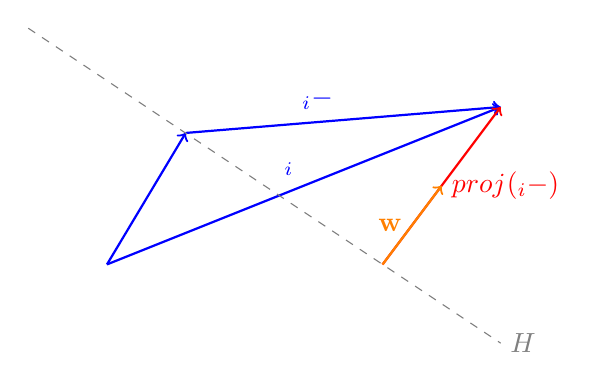
\begin{tikzpicture}
    % Define coordinates
    \coordinate (x) at (0,0);
    \coordinate (xi) at (3,2);
    \coordinate (w) at (1,-1);

    % Draw vector x
    \draw[->, thick, blue] (0,0) -- (1,1.67) node[midway, above left] {$\x$};
    \draw[->, thick, blue] (0,0) -- (5,2) node[midway, above left] {$\x_i$};
    \draw[->, thick, blue] (1,1.67) -- (5,2) node[midway, above left] {$\x_i-\x$};

      % Draw hyperplane
    \draw[dashed, gray] (-1,3) -- (5,-1) node[right] {$H$};

      % Draw projection
    \draw[->, thick, red] (3.5,0) -- (5,2) node[midway, right] {$\text{proj}_{\w}(\x_i - \x)$};

      % Draw vector w
    \draw[->, thick, orange] (3.5,0) -- (4.25,1) node[midway, left] {$\mathbf{w}$};
  \end{tikzpicture}
\end{center}
Simplfiying, we can express this as
\begin{align*}
  \frac{\ip{\x_i-\x}{\w}}{\norm{\w}_2}
   & = \frac{\ip{\x_i}{\w} - \ip{\x}{\w}}{\norm{\w}_2} \tag{linearity}                \\
   & = \frac{\ip{\x_i}{\w} + b}{\norm{\w}_2} \tag{$\x \in H \Harr \ip{\x}{\w}+b = 0$} \\
   & = \frac{\y_i\hat y_i}{\norm{\w}_2}
\end{align*}
We now have something to maximize.
\begin{defn}[margin]
  Given a hyperplane $H := \{\x : \ip{\x}{\w} + b = 0\}$ separating the data,
  the \term{margin} is the smallest distance between a data point $\x_i$ and $H$.

  That is, $\min_i \frac{\y_i \hat y_i}{\norm{\w}_2}$.
\end{defn}
The goal is the maximize the margin across all possible hyperplanes:
\[ \max_{\w,b} \min_i \frac{\y_i \hat y_i}{\norm{\w}_2} \qq{s.t.} \forall i, \y_i \hat y_i > 0 \qq{where} \hat y_i := \ip{\x_i}{\w} + b \]
We claim that we can arbitrarily scale the numerator.
Let $c>0$.
Then, $(\w,b)$ has the same loss as $(c\w,cb)$ because
$\frac{\ip{\x_i}{c\w}+cb}{\norm{c\w}_2}
  = \frac{c\ip{\x_i}{\w}+cb}{c\norm{\w}_2}
  = \frac{\ip{\x_i}{\w}+b}{\norm{\w}_2}$.

Therefore, we can equivalently write
\[ \max_{\w,b} \frac{1}{\norm{\w}_2} \qq{s.t.} \min_i \y_i \hat y_i = 1 \qq{where} \hat y_i := \ip{\x_i}{\w} + b \]
or even better:
\begin{equation}\label{eq:hsvm}
  \min_{\w,b} \norm{\w}_2^2 \qq{s.t.} \forall i,\y_i(\ip{\x_i}{\w} + b) \geq 1
\end{equation}

Finally, consider the points that are closest to the boundary.
\begin{defn*}
  For the separating hyperplane $H = \{\ip{\x_i}{\w}+b = 0\}$,
  the two \term{supporting hyperplanes} are the parallel hyperplanes
  $H_+ := \{\ip{\x_i}{\w}+b = 1\}$ and $H_- := \{\ip{\x_i}{\w}+b = -1\}$
  which represent the margin boundaries.

  A \term{support vector} is a data point $\x_i \in H_+ \cup H_-$.
\end{defn*}
The support vectors are rare, but decisive because they reach the boundary of the constraint.

\paragraph{Explanation from the dual perspective}
Recall the SVM quadratic program
\[ \min_{\w_b} \frac12\norm{\w}^2_2 \qq{s.t.} \forall i,\y_i(\ip{\x_i}{\w}+b) \geq 1 \]
Introduce Lagrangian multipliers (dual variables) $\symbf{\alpha} \in \R^n$.
\begin{align*}
    & \min_{\w,b}\max_{\symbf\alpha>\0} \frac12\norm{\w}^2_2 - \sum_i \alpha_i[\y_i(\ip{\x_i}{\w}+b)-1]                                          \\
  = & \min_{\w,b} \begin{cases}
                    +\infty              & \exists i,\y_i(\ip{\x_i}{\w}+b)<1 (\text{set $\alpha_i$ as $+\infty$})   \\
                    \frac12\norm{\w}_2^2 & \forall i,\y_i(\ip{\x_i}{\w}+b)\geq 1 (\text{set all $\alpha_i$ as $0$})
                  \end{cases} \\
  = & \min_{\w_b} \frac12\norm{\w}^2_2 \qc{s.t.} \forall i,\y_i(\ip{\x_i}{\w}+b) \geq 1
\end{align*}
Therefore, we only need to study the minimax problem.
Assuming that the problem is convex (which it is, outside the scope of the course),
we can express this as
\[
  \max_{\symbf\alpha>\0} \overbrace{\min_{\w,b} \underbrace{\frac12\norm{\w}^2_2 - \sum_i \alpha_i[\y_i(\ip{\x_i}{\w}+b)-1]}_{\Loss(\w,b,\alpha)}}^{\Loss(\alpha)}
\]
and take the derivative of the interior with respect to $\w$ and $b$:
\begin{align*}
  \pdv{\Loss(\w,b,\alpha)}{\w} & = \w - \sum_i \alpha_i \y_i \x_i = 0 \\
  \w^*                         & = \sum_i \alpha_i \y_i \x_i          \\
  \pdv{\Loss(\w,b,\alpha)}{b}  & = - \sum_i \alpha_i \y_i = 0         \\
  \sum_i \alpha_i \y_i         & = 0
\end{align*}
Substitute back into $\Loss(\alpha)$:
\begin{align*}
  \Loss(\alpha)
   & := \min_{\w,b} \frac12\norm{\w}^2_2 - \sum_i \alpha[\y_i(\ip{\x}{\w}+b)-1]                                                                                    \\
   & = \min_{\w,b} \frac12\norm{\w}^2_2 - \ip{\sum_i\alpha_i\y_i\x_i}{\w} - b\sum_i \alpha_i\y_i + \sum_i \alpha_i                                                 \\
   & = \frac12\norm{\sum_i \alpha_i \y_i \x_i}^2_2 - \ip{\sum_i\alpha_i\y_i\x_i}{\sum_i \alpha_i \y_i \x_i} + \sum_i \alpha_i \tag{s.t. $\sum_i \alpha_i\y_i = 0$} \\
   & = -\frac12\norm{\sum_i \alpha_i \y_i \x_i}^2_2 + \sum_i \alpha_i                                                         \tag{s.t. $\sum_i \alpha_i\y_i = 0$}
\end{align*}
Therefore, we can write the dual problem as
\[ \min_{\symbf\alpha\geq0} {-\sum_i \alpha_i} + \frac12 \sum_i\sum_j \alpha_i\alpha_j\y_i\y_j\ip{\x_i}{\x_j} \qq{s.t.} \sum_i \alpha_i\y_i = 0 \]
We prefer this dual problem because it admits a very easy way to
use a non-linear mapping $\x \xto{\phi} \phi(\x)$
to transform non-linearly separable data $\x$
into linearly separable $\phi(\x)$.
After applying the unknown non-linear mapping, we get
\[ \min_{\symbf\alpha\geq0} {-\sum_i \alpha_i} + \frac12 \sum_i\sum_j \alpha_i\alpha_j\y_i\y_j\textcolor{blue}{\ip{\phi(\x_i)}{\phi(\x_j)}} \qq{s.t.} \sum_i \alpha_i\y_i = 0 \]
which we can find \emph{without explicitly applying $\phi$}
by using the ``kernel trick'' from \cref{ch:kernel},
writing the \textcolor{blue}{inner product} directly as a non-linear function.

\section{Soft-Margin Support Vector Machines}\label{ch:ssvm}
\lecture{Jan 30}

One of the drawbacks of the hard-margin SVM is that the data must be linearly separable.
That is, there must exist a non-zero margin between the data.

If we have a small number of outliers on the wrong side of the decision boundary,
we can instead just penalize it in the loss.
We do this by relaxing the constraint in hard-margin SVM
and including failures in the objective function.

\begin{defn}[hinge loss]
  Given label $\y \in \{-1,+1\}$ and score $\hat y := \ip{\x}{\w}+b$,
  let $\y\hat y$ be the confidence.

  Define $\ell_{\hinge} = (1-\y\hat y)^+ = \begin{cases}
      1-\y\hat y & \y\hat y < 1     \\
      0          & \text{otherwise}
    \end{cases}$
\end{defn}

In general, notate $x^+$ to mean $\max\{x,0\}$.

Now, we can formulate the soft-margin SVM as
\begin{equation}\label{eq:ssvm}
  \boxed{
    \min_{\w,b} \textcolor{blue}{\frac12\norm{\w}^2_2}
    + \textcolor{orange}{C} \cdot \textcolor{red}{\sum_i(1-\y_i\hat y_i)^+}
    \qq{s.t.} \hat y_i = \ip{\x_i}{\w}+b
  }
\end{equation}
(\textcolor{blue}{margin maximization}, \textcolor{orange}{regularization hyperparameter}, \textcolor{red}{error penalty}).
Notice that the hard-margin SVM is the limiting behaviour
of the soft-margin SVM as $C \to \infty$.

\paragraph{Why do we use the hinge loss?}
Consider the probability that $\Y \neq \sgn(\hat \Y)$
\begin{align*}
  \Pr[\Y \neq \sgn(\hat \Y)]
  = \Pr[\Y\hat\Y \leq 0]
  = \E[\I[\Y\hat\Y \leq 0]]
  =: \E[\ell_{0-1}(\Y\hat\Y)]
\end{align*}
We want to minimize $\E[\ell_{0-1}(\Y\hat\Y)]$.
Minimizing this value is hard because $\ell_{0-1}$ is discontinuous at 0
and has gradient $\vb 0$ almost everywhere.

By Bayes' rule, we can rewrite as
$\E_{\vv X}\E_{\Y \mid \vv X}[\ell_{0-1}(\Y\hat\Y)]$.
Then, we can minimize instead
\[ \eta(\x) = \argmin_{\hat y \in \R} \E_{\Y \mid \vv X=\x}[\ell_{0-1}(\Y\hat y)] \]
since setting $\Y = \eta(\vv X)$.

\begin{defn}[classification calibrated]
  We say a loss function $\ell(\y\hat y)$ is \term{classification calibrated}
  if for all $\x$,
  \[ \hat\y(\x) := \argmin_{\hat y \in \R}\E_{\Y \mid \vv \X=\x}[\ell(Y\hat y)] \]
  has the same sign as the Bayes rule $\eta(\x)$.
\end{defn}

Due to Bartlett, we have a helpful theorem
\begin{theorem}[characterization under convexity]
  Any convex loss $\ell$ is classification calibrated if and only if
  $\ell$ is differentiable at 0 and $\ell'(0) < 0$.
\end{theorem}
\begin{corollary}
  A classifier that minimizes the expected hinge loss
  also minimizes the expected 0-1 loss.
\end{corollary}

This theorem is also one of the big reasons why the perceptron
cannot generalize well.

\begin{remark}
  The perceptron loss $\ell(\y\hat y) = -\min\{\y\hat y,0\}$
  is not differentiable at 0,
  so it is not classification calibrated and cannot generalize.
\end{remark}

\paragraph{Generating the dual}
Recall the soft-margin SVM
\[
  \min_{\w,b} \frac12\norm{\w}^2_2
  + C\cdot \sum_i(1-\y_i(\ip{\x_i}{\w}+b))^+
\]
Notice that we can write
$C\cdot(t)^+ = \max\{Ct,0\} = \max_{0 \leq \alpha \leq C} \alpha t$
to get
\[
  \min_{\w,b} \max_{0 \leq \symbf{\alpha} \leq C}
  \frac12\norm{\w}^2_2
  + \sum_i\alpha_i(1-\y_i(\ip{\x_i}{\w}+b))
\]
As before, swap min with max:
\[
  \max_{0 \leq \symbf{\alpha} \leq C} \overbrace{
    \min_{\w,b} \underbrace{
      \frac12\norm{\w}^2_2 + \sum_i\alpha_i(1-\y_i(\ip{\x_i}{\w}+b))
    }_{\Loss(\w,b,\alpha)}
  }^{\Loss(\alpha)}
\]
Now, set our optimality conditions
\begin{align*}
  \pdv{\Loss(\w,b,\alpha)}{\w} & = \w - \sum_i \alpha_i \y_i \x_i = \vb 0 &
  \pdv{\Loss(\w,b,\alpha)}{b}  & = -\sum_i \alpha_i \y_i = 0                \\
  \w                           & = \sum_i \alpha_i \y_i \x_i              &
  \sum_i\alpha_i\y_i           & = 0
\end{align*}
and substitute into $\Loss(\alpha)$:
\begin{align*}
  \Loss(\alpha)
   & := \frac12\norm{\w}^2_2 + \sum_i\alpha_i(1-\y_i(\ip{\x_i}{\w}+b))                              \\
   & = \frac12\norm{\sum_i \alpha_i \y_i \x_i}^2_2 + \sum_i\alpha_i - \ip{\sum_i \alpha_i \y_i\x_i} \\
   & = -\frac12\norm{\sum_i \alpha_i \y_i \x_i}^2_2 + \sum_i \alpha_i
\end{align*}
Switching from max to min and expanding the norm, we get
\begin{equation}\label{eq:ssvmd}
  \boxed{
    \min_{0 \leq \symbf{\alpha} \leq C}
    -\sum_i \alpha_i +
    \frac12 \sum_i \sum_j \alpha_i \alpha_j y_i y_j \ip{\x_i}{\x_j}
    \qq{s.t.}
    \sum_i \alpha_i \y_i = 0
  }
\end{equation}
which is identical to the hard-margin SVM dual with an upper bound $C$ on $\symbf\alpha$.

\lecture{Feb 1}

Suppose we solve the dual (\cref{eq:ssvmd}) with optimal solution $\symbf\alpha^*$.
Then,
\begin{equation}\label{eq:ssvmw}
  \w^* = \sum_i \alpha^*_i \y_i \x_i.
\end{equation}
If we have a point on $H_{\pm 1}$, i.e., $\y\hat y = 1$,
we can recover $b^*$ as $\y - \ip{\x}{\w^*}$.

\paragraph{Training by gradient descent}
Suppose we have a minimization problem $\min_{\x} f(\x)$.
Then, to make a guess $\x$ better, set $\x \gets \x - \eta \cdot \nabla_{\x} f(\x)$
for some \term{learning rate} $\eta > 0$.

Given the problem
\[
  \min_{\w,b} \frac{1}{2\lambda} \norm{\w}_2^2 + C\sum_i \ell(\y_i\hat y_i)
  \qq{where}
  \hat y_i = \ip{\x_i,\w} + b
\]
with loss function $\ell$, the gradient descent steps are
\begin{align*}
  \w & \gets \w - \eta \cdot \nabla_{\w}\qty(\frac{1}{2\lambda} \norm{\w}_2^2 + C\sum_i \ell(\y_i\hat y_i)) \\
     & = \w - \eta \qty[\frac{\w}{\lambda} + C\sum_i \ell'(\y_i\hat y_i)\y_i\x_i]                           \\
  b  & \gets b - \eta \cdot \nabla_b\qty(\frac{1}{2\lambda} \norm{\w}_2^2 + C\sum_i \ell(\y_i\hat y_i))     \\
     & = b - \eta \qty[C\sum_i \ell'(\y_i \hat y_i)\y_i]
\end{align*}
because $\nabla_{\w} \ell(\y_i\hat y_i) = \ell'(\y_i\hat y_i)\cdot\y_i\nabla_{\w}(\hat y_i) = \ell'(\y_i\hat y_i)\y_i\x_i$
and $\nabla_b \ell(\y_i\hat y_i) = \ell'(\y_i\hat y_i)\cdot\y_i \nabla_b(\hat y_i) = \ell'(\y_i\hat y_i)\cdot \y_i$.

If $\ell$ is hinge loss, we define the derivative $\ell'(t) = \begin{cases}
    -1 & t \leq 1 \\
    0  & t > 1
  \end{cases}$.

If $\ell$ is perceptron loss, we define $\ell'(t) = \begin{cases}
    -1 & t \leq 0 \\
    0  & t > 1
  \end{cases}$.

All other common loss functions are easily differentiable.

\section{Reproducing Kernels}\label{ch:kernel}
\newcommand{\phix}[1]{\mqty[\vec{#1#1\trans} \\ \sqrt{2}#1 \\ 1]}

We have dealt with data that is perfectly linearly separable (hard-margin SVM)
and mostly linearly separable (soft-margin SVM).

\begin{problem}
  How can we use our existing techniques to classify
  a fully non-linearly separable dataset?
\end{problem}

In the linear classifier, we used an affine function $\ip{\w}{\x}+b$.
Now, we define a quadratic classifier.

\begin{defn}[quadratic classifier]
  A function $f : \R^d \to \R^d$ of the form $f(\x) = \ip{\x}{Q\x} + \sqrt{2}\ip{\x}{\p} + b$
  where the weights to be learned are $Q \in \R^{d\times d}$, $\p \in \R^d$, and $b \in \R$.
\end{defn}

Recall from linear algebra that for all $A$, $B$, $C$, $\ip{AB}{C} = \ip{B}{A\trans C}$
and $\ip{A}{BC} = \ip{AB\trans}{C}$.

\begin{defn}[matrix vectorization]
  Given a matrix $\vb{A} \in \R^{m\times n}$,
  let $\vec{\vb{A}} \in \R^{mn}$ be its vectorization.
  That is,
  \[
    \vb A = \mqty[a_{11} & a_{12} & \cdots & a_{1n} \\ a_{21} & a_{22} & \cdots & a_{2n} \\ \vdots & \vdots & \ddots & \vdots \\ a_{m1} & a_{m2} & \cdots & a_{mn}]
    \implies
    \vec{\vb A} = \mqty[a_{11} \\ a_{12} \\ \vdots \\ a_{1n} \\ \vdots \\ a_{mn}]
  \]
\end{defn}

Then, we can write the quadratic classifier as:
\begin{align*}
  f(\x) & =  \ip{\x}{Q\x} + \sqrt{2}\ip{\x}{\p} + b       \\
        & =  \ip{\x\x\trans}{Q} + \ip{\sqrt{2}\x}{\p} + b \\
        & = \ip{\phix{\x}}{\bmqty{\vec{Q}                 \\\p\\b}}
\end{align*}
If we write $\phi(\x) = (\vec{\x\x\trans}, \sqrt{2}\x, 1)\trans$
and $\w = (\vec{Q}, \p, b)\trans$,
then we can write $f$ as
\[ f(\x) = \ip{\phi(\x)}{\w} \]
but this really blows up the dimension to $\R^{d^2+d+1}$.
Recall that in the dual forms of SVM,
all we need is to know the inner product $\ip{\phi(\x)}{\phi(\w)}$.
With our new $\phi$, we get
\begin{align*}
  k(\x,\z) := \ip{\phi(\x)}{\phi(\z)}
   & = \ip{\phix{\x}}{\phix{\z}}                                             \\
   & = \ip{\vec{\x\x\trans}}{\vec{\z\z\trans}} + \ip{\sqrt2\x}{\sqrt2\z} + 1 \\
   & = \ip{\x}{\z}^2 + 2\ip{\x}{\z} + 1                                      \\
   & = (\ip{\x}{\z} + 1)^2
\end{align*}

This process is easily reproducable for a given $\phi$.
What about the other direction?

\begin{defn}[reproducing kernel]
  We call $k : \mathcal{X} \times \mathcal{X} \to \R$
  a \term{reproducing kernel} if there exists some $\phi : \mathcal{X} \to \mathcal{H}$
  so that $\ip{\phi(\x)}{\phi(\z)} = k(\x,\z)$.
\end{defn}

\begin{remark}
  When such a kernel exists, it may not be unique.

  For example, the kernels $\phi(\x) = [x_1^2,\sqrt2 x_1x_2,x_2^2] \in \R^3$
  and $\psi(\x) = [x_1^2,x_1x_2,x_1x_2,x_2^2] \in \R^4$
  have the same inner product $\ip{\phi(\x)}{\phi(\z)} = \ip{\psi(\x)}{\psi(\z)}$.
\end{remark}

\begin{theorem}[Mercer's theorem]
  $k : \mathcal{X} \times \mathcal{X} \to \R$ is a kernel if and only if
  for any $n \in \N$ and any $\x_1,\dotsc,\x_n \in \mathcal{X}$,
  the \term{kernel matrix} $K_{ij} := k(\x_i,\x_j)$ is symmetric and positive semi-definite.
\end{theorem}

Recall from linear algebra: $K$ is \term{symmetric} if $K_{ij} = K_{ji}$ for all indices,
and \term{positive semi-definite} if $\ip{\symbf\alpha}{K\symbf\alpha} \geq 0$ for all vectors $\symbf\alpha$.

The proof is extremely convoluted and well beyond the scope of the course.

\begin{example}
  The following are kernels:
  \begin{itemize}
    \item the polynomial kernel $k(\x,\z) = (\ip{\x}{\z} + 1)^p$ for hyperparameter $p$,
    \item the Gaussian kernel $k(\x,\z) = \exp(-\norm{\x-\z}_2^2/\sigma)$ for hyperparameter $\sigma$, and
    \item the Laplace kernel $k(\x,\z) = \exp(-\norm{\x-\z}_2/\sigma)$ for hyperparameter $\sigma$
  \end{itemize}
\end{example}

Now, we can substitute our expression for the inner product to \cref{eq:ssvm,eq:ssvmd},
the primal and dual of the soft-margin SVM:
\begin{gather*}
  \min_{\w,b} \frac12\norm{\w}_2^2 + C\cdot\sum_i(1-\y_i\hat y_i)^+
  \qq{s.t.} \hat y_i = \ip{\phi(\x_i)}{\w} \\
  \min_{0 \leq \symbf{\alpha} \leq C}
  -\sum_i \alpha_i + \frac12 \sum_i \sum_j \alpha_i \alpha_j y_i y_j k(\x_i,\x_j)
  \qq{s.t.} \sum_i \alpha_i \y_i = 0
\end{gather*}

Once we solve $\symbf\alpha^*$, we can try to recover $\w^*$ as in \cref{eq:ssvmw}
\[ \w^* = \sum \alpha_i^*\y_i \phi(\x_i) \]
but this will not work since we do not know $\phi$ explicitly.
Instead, we only need to compute the score function
\begin{align*}
  f(\x) & := \ip{\phi(\x)}{\w^*}                          \\
        & = \ip{\phi(\x)}{\sum \alpha_i^*\y_i \phi(\x_i)} \\
        & = \sum \alpha_i^*\y_i \ip{\phi(\x)}{\phi(\x_i)} \\
        & = \sum \alpha_i^*\y_i k(\x,\x_i)
\end{align*}
and return $\sgn(f(\x))$.

\section{Gradient Descent}\label{ch:gd}
\lecture{Feb 6}

All of our machine learning models so far have been expressed as optimization problems
(\cref{eq:lgr,eq:hsvm,eq:ssvm}).
\begin{remark}
  Optimization problems are identical up to constants.
  That is,
  \[ \min_{\x} f(\x) = \min_{\x} c\cdot f(x) \]
  if $c$ has no $\x$-dependence.
\end{remark}
We can consider now a generic optimization problem $\min\limits_{\x} f(\x)$.

Assume that $f(\x)$ is differentiable with gradient $\nabla_{\x} f(\x)$.
\begin{notation}
  Given the generic optimization problem,
  write $f^* := \min_{\x} f(x)$ for the optimal value
  and $x^* := \argmin_{\x} f(x)$ for the optimal parameter.
\end{notation}
Then, we can define gradient descent.
\begin{definition}[gradient descent]
  Choose an initial point $\x^{(0)} \in \R^d$ and repeat
  \[ x^{(k)} = x^{(k-1)} - \underbrace{t}_{\mathclap{\text{step size}}} \cdot \nabla f(x^{(k-1)}) \]
  $k = 1,2,\dotsc$ for some step size $t > 0$ until satisfied.
\end{definition}
Intuitively, we are walking ``down'' the function by checking
for a downwards slope and taking a $t$-sized step down that slope.

For example, the perceptron (\cref{ch:p}) with optimization problem
\[
  \min_{\w}f(\w) = \min_{\w} -\frac1n\sum_i\y_i\ip{\w}{\x_i}\I[\text{mistake on $\x_i$}]
\]
with gradient
\[
  \nabla_{\w} f(\w) = -\frac1n\sum_i\y_i\x_i\I[\text{mistake on $\x_i$}]
\]
leads us to the gradient descent update
\[
  \w \gets \w + t\qty[\frac1n\sum_i\y_i\x_i\I[\text{mistake on $\x_i$}]]
\]
This is very expensive, since we need to iterate over our entire training data
for each update.
Since the gradient is just a sample mean, we can make an estimation
\[
  \widetilde{\nabla_{\w}f(\w)} = \y_I\x_I\I[\text{mistake on $\x_I$}]
\]
after picking a random index $I \in_{\vv R} \{1,\dotsc,n\}$.
This is an unbiased estimator of the sample mean.
Doing this, i.e.,
\[ \w \gets \w + t\y_I\x_I\I[\text{mistake on $\x_I$}] \]
is called \term{stochastic gradient descent}.
Since it is (very) inaccurate, it will take many more iterations to converge.

For a more complex example, consider the soft-margin SVM (\cref{ch:ssvm})
with optimization problem
\[
  \min_{\w,b} \frac12\norm{\w}^2_2 + C\sum_i \ell_{\vv{hinge}}(1-\y_i\hat y_i)
  \qq{s.t.} \hat y_i = \ip{\x_i}{\w}+b
\]
We calculate two gradients $\nabla_{\w}$ and $\nabla_b$ to get
\begin{align*}
  \w & \gets \w - t\qty[\w + C\sum_i \ell'_{\vv{hinge}}(\y_i\hat y_i)\y_i\x_i] \\
  b  & \gets b - t\qty[C\sum_i \ell'_{\vv{hinge}}(\y_i\hat y_i)\y_i]
\end{align*}

\paragraph{Motivating gradient descent}
Suppose we take the Taylor expansion of $f$ at the current iterate $\x$.
Then, we can say
\[ f(\vb y) \approx f(\x) + \nabla f(\x)\trans(\vb y-\x) + \frac1{2t}\norm{\vb y-\x}_2^2 \]
and take the minimization with respect to $\vb y$ on both sides
\[
  \min_{\vb y} f(\vb y) \approx
  \min_{\vb y}\qty[\underbrace{f(\x) + \nabla f(\x)\trans(\vb y-\x) + \frac1{2t}\norm{\vb y-\x}_2^2}_{g(\vb y)}]
\]
so that we can write
\begin{align*}
  \pdv{g}{\vb y} = 0 + \nabla f(\x) + \frac1t(y-x) & = 0                  \\
  t\nabla f(\x) + \vb y- \x                        & = 0                  \\
  \vb y                                            & = \x - t\nabla f(\x)
\end{align*}
which is our gradient descent formula.

\paragraph{Applying gradient descent}
We cannot set the step size too large (it will diverge)
or too small (it will be too slow). How do we choose the step size?

\begin{defn}[convexity]
  A function $f$ is \term*{convex} if $f(\vb y) \geq f(\x) + \nabla f(\x)\trans(\vb y-\x)$
  for any $\x,\vb y \in \R^d$.
\end{defn}
We also want to characterize the smoothness.
\begin{defn}[Lipschitz continuity]
  Given convex and differentiable $f$, we say $f$ is \term*{$L$-smooth}
  or \term*{$L$-Lipschitz continuous} for $L > 0$ if the matrix
  \[ LI - \nabla^2f(\x) \]
  is positive semi-definite for every $x$ (we write $LI \succeq \nabla^2 f(x)$).
\end{defn}
Then, we can characterize the convergence rate.
\begin{theorem}[convergence rate for convex case]
  Gradient descent with fixed step size $t \leq 1/L$ satisfies
  \[
    f(\x^{(k)}) - f^* \leq \frac{\norm{\x^{(0)} - \x^*}_2^2}{2tk}
  \]
  We say gradient descent has convergence rate $\order{1/k}$
  (i.e., a bound of $f(\x^{(k)}) - f(\x^*) \leq \varepsilon$
  takes $\order{1/\varepsilon}$ iterations).
\end{theorem}
\begin{prf}
  Recall the mean value theorem allows us to write the Lagrangian
  \[
    f(\vb y) = f(\x) + \nabla f(\x)\trans(\vb y - \x) + \frac12(\vb y - \x)\trans\nabla^2 f(\vb a)(\vb y-\x)
  \]
  where $\vb a$ is on the line between $\vb x$ and $\vb y$.
  Then, since $LI \succeq \nabla^2 f(\vb a)$, we have
  \begin{align*}
    f(\vb y)
     & \leq f(\x) + \nabla f(\x)\trans(\vb y - \x) + \frac{L}2(\vb y - \x)\trans(\vb y-\x) \\
     & \leq f(\x) + \nabla f(\x)\trans(\vb y - \x) + \frac{L}2\norm{\vb y - \x}_2^2
  \end{align*}
  Now, plug in $\vb y = \x^+ := \x - t\nabla f(\x)$ (i.e., do the gradient update) to get
  \begin{align*}
    f(\x^+)
     & \leq f(\x) + \nabla f(\x)\trans(\x - t\nabla f(\x) - \x) + \frac{L}2\norm{\x - t(\nabla f(\x)) - \x}_2^2 \\
     & = f(\x) - t\norm{\nabla f(\x)}_2^2 + \frac{Lt^2}2\norm{\nabla f(\x)}_2^2                                 \\
     & = f(\x) - (1-\frac12 Lt)t\norm{\nabla f(\x)}_2^2
  \end{align*}
  Since $t \leq \frac1L$, we have $(1-\frac12Lt) \geq \frac12$ and we can conclude that
  \[
    f(\x^+) \leq f(\x) - \frac12t\norm{\nabla f(\x)}^2_2 \tag{$\star$}
  \]
  which means that we have decreased the function value by at least $\frac{t}{2}\norm{\nabla f(\x)}_2^2$.

  Recall that $f$ is convex.
  Then, by definition, $f(\x^*) \geq f(\x) + \nabla f(\x)\trans(\x^* - \x)$.
  Equivalently,
  \[ f(\x) \leq f(\x^*) + \nabla f(\x)\trans(\x-\x^*) \]
  and by ($\star$) we can say
  \begin{align*}
    f(\x^+)           & \leq f(\x^*) + \nabla f(\x)\trans(\x-\x^*) - \frac{t}{2}\norm{\nabla f(\x)}_2^2                                          \\
    f(\x^+) - f(\x^*) & \leq \nabla f(\x)\trans(\x-\x^*) - \frac{t}{2}\norm{\nabla f(\x)}_2^2                                                    \\
                      & = \frac1{2t}\qty(2t\nabla f(\x)\trans(\x-\x^*) - t^2\norm{\nabla f(\x)}_2^2)                                             \\
                      & = \frac1{2t}\qty((2t\nabla f(\x)\trans(\x-\x^*) - t^2\norm{\nabla f(\x)}_2^2 - \norm{\x-\x^*}_2^2) + \norm{\x-\x^*}_2^2) \\
                      & = \frac1{2t}\qty(-\norm{\x-t\nabla f(\x)-\x^*} + \norm{\x-\x^*}_2^2)                                                     \\
                      & = \frac1{2t}\qty(\norm{\x-\x^*}_2^2 - \norm{\x^+ - \x^*}_2^2)
  \end{align*}
  If we define $\x^+ := \x^{(i)}$ and $\x := \x^{(i-1)}$, we have
  \begin{align*}
    f(\x^{(i)}) - f(\x^*)
     & \leq \frac{1}{2t}\qty(\norm{\x^{(i-1)}-\x^*}_2^2 - \norm{\x^{(i)} - \x^*}_2^2)              \\
    \sum_{i=1}^k \qty[f(\x^{(i)}) - f(\x^*)]
     & \leq \sum_{i=1}^k \frac{1}{2t}\qty(\norm{\x^{(i-1)}-\x^*}_2^2 - \norm{\x^{(i)} - \x^*}_2^2) \\
    \sum_{i=1}^k f(\x^{(i)}) - k f(\x^*)
     & \leq \frac{1}{2t}\qty(\norm{\x^{(0)}-\x^*}_2^2 - \norm{\x^{(k)} - \x^*}_2^2)                \\
     & \leq \frac{1}{2t}\qty(\norm{\x^{(0)}-\x^*}_2^2)                                             \\
    \frac1k\sum_{i=1}^k f(\x^{(i)}) - f(\x^*)
     & \leq \frac{1}{2tk}\qty(\norm{\x^{(0)}-\x^*}_2^2)
  \end{align*}
  Finally, because each step decreases, we must have $f(\x^{(k)}) \leq \frac1k\sum_{i=1}^k f(\x^{(i)})$.
  That is,
  \begin{align*}
    f(\x^{(k)}) - f^* \leq \frac1k\sum_{i=1}^k f(\x^{(i)}) - f(\x^*) \leq \frac{1}{2tk}\qty(\norm{\x^{(0)}-\x^*}_2^2)
  \end{align*}
  as desired.
\end{prf}

\lecture{Feb 8}
We have a stronger sense of convexity that gives a stronger convergence rate.

\begin{defn}[$m$-strong convexity]
  For some $m > 0$, $f$ is \term*{$m$-strong convex}
  if $f(\x) - m\norm{\x}_2^2$ is convex.
  We write $LI \succeq \nabla^2f(\x) \succeq mI$.
\end{defn}

\begin{theorem}[convergence rate for strong convexity]
  Let $f$ be differentiable, $m$-strong convex, and $L$-smooth.
  Then, gradient descent with fixed step size $t \leq 2/(m+L)$ satisfies
  \[ f(\x^{(k)}) - f^* \leq \gamma^k\frac{L}{2}\norm{\x^{(0)}-\x^*}_2^2 \]
  where $0 < \gamma < 1$.
\end{theorem}

The rate here is $\order{\gamma^k}$ which is exponentially fast.
That is, a bound $f(\x^{(k)}) - f(\x^*) < \varepsilon$
can be achieved using only $\order{\log_{1/\gamma}(1/\varepsilon)}$ iterations,
much better than before.

Alternatively, we can make a weaker assumption and ask for a weaker result.
In a non-convex function, there are (potentially many) local minima.
Instead of asking for small $\norm{f(\x^{(k)}) - f(\x^*)}_2$,
we only need $\norm{\nabla f(\x)}$.

\begin{theorem}[convergence rate for non-convex case]
  Suppose $f$ is differentiable, $L$-smooth, and non-convex.
  Then, gradient descent with fixed step size $t \leq 1/L$ satisfies
  \[ \min_{i=0,\dotsc,k} \norm{\nabla f(\x^{(i)})}_2 \leq \sqrt{\frac{2(f(\x^{(0)}) - f^*)}{t(k+1)}} \]
\end{theorem}

The rate $\order{1/\sqrt{k}}$ for finding stationary points cannot be improved
by any deterministic algorithm.

However, all these require that the gradient $\nabla f(\x)$ is known to us.

\paragraph{Stochastic gradient descent}
Recall that we introduced the case for perceptron where we update using one data point
instead of the full dataset.

Consider some decomposable optimization with unreasonably large $n$
\[ \min_{\w} \frac1n\sum_i f_i(\w) \]
where we assume $\nabla f_i(\w)$ exists for all $i$.
Then, the two gradient descent updates
\begin{align*}
  \w & \gets \w - t\frac1n\sum_i \nabla f_i(\w) \\
  \w & \gets \w - t \cdot \nabla f_I(\w)
\end{align*}
(where $I$ is a uniformly random index) have the same expected value.
Notice that the ``full'' gradient descent will have true time complexity
$\order{n/\varepsilon}$ because each step takes $\order{n}$ time to calculate.

The stochastic version takes just $\order{1/\varepsilon^2}$ time.

To summarize these theorems:
\begin{center}
  \begin{tabular}{r|CCC}
    Case              & \text{Hessian assumption}            & \text{Iterations for $\varepsilon$ error} & \text{Step size} \\ \hline
    Non-convex        & LI \succeq \nabla^2 f(\x)            & \order{1/\varepsilon^2}                   & t \leq 1/L       \\
    Convex            & LI \succeq \nabla^2 f(\x)            & \order{1/\varepsilon}                     & t \leq 1/L       \\
    $m$-strong convex & LI \succeq \nabla^2 f(\x) \succeq mI & \order{\log(1/\varepsilon)}               & t \leq 2/(m+L)   \\
    Stochastic convex & LI \succeq \nabla^2 f(\x)            & \order{1/\varepsilon^2}                   & t = 1/k
  \end{tabular}
\end{center}

In general, we will want to use stochastic gradient descent when $n > C_1/\varepsilon$
and full gradient descent when $n < C_2/\varepsilon$ for some constants $C_1$, $C_2$.

\chapter{Neural Networks}

We can finally progress from 30- to 60-year old algorithms to stuff people actually use now.
Recall the XOR dataset (\cref{exa:xor}).
We showed that it is not linearly separable, so it cannot be learned by perceptron (\cref{thm:perceptron-fail}).

One way to deal with this is to use a richer model (e.g., a quadratic classifier)
or to lift the data through some feature map $\phi$.
These two approaches are equivalent due to reproducing kernels.

A neural network tries to learn the feature map \emph{and} the linear classifier simultaneously.

\section{Multilayer Perceptron}

We can set up the following layers:
\begin{itemize}[nosep]
  \item \term{input layer} $\vb x \in \R^2$
  \item \term{linear layer} $\z = \U\x + \vb c$ for learnable parameters $\U \in \R^{2\times 2}$ and $\vb c \in \R^2$
  \item \term{hidden layer} $\h = \sigma(\z)$ for some non-linear $\sigma$
  \item \term{prediction layer} $\hat y = \ip{\h}{\w} + b$ for learnable parameters $\w \in \R^2$ and $b \in \R$
  \item \term{output layer} $\sgn(\hat y)$ or $\sigmoid(\hat y)$
\end{itemize}
In total, we need to learn $\U$, $\vb c$, $\vb w$, and $b$ (here, 9 parameters).

\begin{example}
  XOR dataset is learnable with a 2-layer neural network. Let
  \[ \U = \mqty[1&1\\1&1] \qc \vb c = \mqty[0\\-1] \qc \w = \mqty[2\\-4] \qc b = -1 \]
  and let $\sigma(t) = \max\{t,0\}$ (the ReLU activation function).

  Then, $\sgn(\ip{\sigma(\U\x+\vb c)}{\w} + b)$ works.
\end{example}

To do a multi-class classification, simply have a bunch of $\hat y$'s in a vector
$\hat{\vb y} = \W\h + \vb b$ and make a prediction vector $\hat{\p} = \softmax(\hat{\vb y})$.

\begin{remark}
  The hidden layer $\sigma$ \emph{must} be non-linear.
  Otherwise, the composition of linear layers is just a linear layer and we gain nothing.
\end{remark}

There are a lot of options for $\sigma$:
\begin{itemize}[nosep]
  \item $\xx{relu}(t) = t_+$
  \item $\xx{elu}(t) = t_+ + t_-(\exp(t)-1)$
  \item $\xx{sgm}(t) = 1/(1+\exp(-t))$
  \item $\tanh(t) = 1-2\xx{sgm}(t)$
\end{itemize}

We can also stack several layers together,
repeating the pattern of linear layer + non-linear layer.

To train, we need a loss function $\ell$ and a dataset $\mathcal D = \{ (\x_i,\y_i) \}$

\begin{notation}
  Write $[\ell \circ f](\x_i,\y_i,\w)$ to mean $\ell[f(\x_i,\w),\y_i]$.
\end{notation}

We can express the neural network as a minimization problem
\begin{equation}
  \min_{\w} \frac1n \sum_i [\ell \circ f](\x_i,\y_i,\w)
\end{equation}
which gives the gradient descent rule
\[
  \w \gets \w - \eta \cdot \frac1n \sum_i \nabla[\ell \circ f](\x_i,\y_i,\w)
\]
for learning rate $\eta$.
This requires a full pass over the dataset for each step.

Instead of doing ordinary stochastic gradient descent,
we can \term{minibatch} by picking a random subset $B \subseteq \{1,\dotsc,n\}$:
\[
  \w \gets \w - \eta \cdot \frac{1}{\abs{B}} \sum_{i \in B} \nabla[\ell \circ f](\x_i,\y_i,\w)
\]
which trades off variance and computation cost.

\lecture{Feb 13}

The learning rate has diminishing returns.
Instead of keeping a constant $\eta$, we can paramaterize $\eta_t$
and say something like
\[
  \eta_t = \begin{cases}
    \eta_0     & t \leq t_0       \\
    \eta_0/10  & t_0 < t \leq t_1 \\
    \eta_0/100 & t_1 < t
  \end{cases}
\]
for an initial $\eta_0$ and specific epochs $t_0,t_1$.
Alterntaively, we can use \term{sublinear decay} $\eta_t = \eta_0/(1+ct)$
or $\eta_t = \eta_0/\sqrt{1+ct}$ for some constant $c$.

We need to calculate a lot of partial derivatives with respect to matrices.
\begin{defn}
  Let $y(\X) \in \R$ and $\X = [X_{ij}] \in \R^{m \times n}$.
  Then, we define the \term*{partial derivative of $y$ w.r.t.~$\X$} as
  \[
    \pdv{y}{\X} = \qty[\pdv{y}{X_{ij}}] = \begin{bmatrix}
      \pdv{y}{X_{11}} & \pdv{y}{X_{12}} & \cdots & \pdv{y}{X_{1n}} \\
      \pdv{y}{X_{21}} & \pdv{y}{X_{22}} & \cdots & \pdv{y}{X_{2n}} \\
      \vdots          & \vdots          &        & \vdots          \\
      \pdv{y}{X_{m1}} & \pdv{y}{X_{m2}} & \cdots & \pdv{y}{X_{mn}}
    \end{bmatrix} \in \R^{m \times n}
  \]
  as a matrix.
\end{defn}
The best way to do this is to just ``guess'' analogous to scalar calculus,
then check that the dimension is right (i.e., $\fn{dim} \pdv{y}{\X} = \fn{dim} \X$)

Consider the forward pass for NN width $k$ and output dimension $c$:
\begin{align*}
  \x    & = \text{input}                   &  & \x \in \R^{d\times 1}                                    \\
  \z    & = \W\x + \vb b_1                 &  & \W \in \R^{k \times d},\ \z,\vb b_1 \in \R^{k \times 1}  \\
  \vb h & = \ReLU(\z)                      &  & \vb h \in \R^{k \times 1}                                \\
  \vth  & = \U\h + \vb b_2                 &  & \U \in \R^{c\times k},\ \vth,\vb b_2 \in \R^{c \times 1} \\
  J     & = \frac12\norm{\vth - \vb y}_2^2 &  & \y \in \R^{c \times 1},\ J \in \R
\end{align*}

Now, we can apply the chain rule to find our desired gradients:
\begin{align*}
  \pdv{J}{\vth}    & = \vth - \vb y                                                                                                                                                                 \\
  \pdv{J}{\U}      & = \pdv{J}{\vth} \circ \pdv{\vth}{\U} = \underbrace{(\vth - \vb y)}_{c \times 1}\underbrace{\vb h\trans}_{1 \times k} \tag{to get $c\times k$}                                  \\
  \pdv{J}{\vb b_2} & = \pdv{J}{\vth} \circ \pdv{\vth}{\vb b_2} = \underbrace{\vth - \vb y}_{c \times 1} \tag{already has right dimensions}                                                          \\
  \pdv{J}{\vb h}   & = \pdv{J}{\vth} \circ \pdv{\vth}{\vb h} = \underbrace{\U\trans}_{k \times c}\underbrace{(\vth - \vb y)}_{c \times 1} \tag{to get $k \times 1$}                                 \\
  \pdv{J}{\vb z}   & = \pdv{J}{\vb h} \circ \pdv{\vb h}{\z} = \underbrace{\U\trans(\vth - \vb y)}_{k \times 1} \odot \underbrace{\ReLU'(\z)}_{k \times 1} \tag{using $\odot$ to keep the dimension} \\
  \pdv{J}{\W}      & = \pdv{J}{\z} \circ \pdv{\z}{\W} = \underbrace{(\U\trans(\vth - \vb y)\odot\ReLU'(\z))}_{k \times 1}\underbrace{\x\trans}_{1 \times d} \tag{to get $k \times d$}               \\
  \pdv{J}{\vb b_1} & = \pdv{J}{\z} \circ \pdv{\z}{\vb b_1} = \underbrace{(\U\trans(\vth - \vb y)\odot\ReLU'(\z))}_{k \times 1} \tag{already has right dimensions}
\end{align*}
where $\odot$ is the Hadamard (element-wise) product, i.e.,
\[
  \mqty[a_1\\a_2\\\vdots\\a_d] \odot \mqty[b_1\\b_2\\\vdots\\b_d] = \mqty[a_1b_1\\a_2b_2\\\vdots\\a_db_d]
\]
for two matrices of identical dimension.

Existing frameworks like TensorFlow will automatically do this.

\begin{theorem}[universal approximation theorem by 2-layer NNs]
  For any continuous function $f : \R^d \to \R^c$ and any $\varepsilon > 0$,
  there exists $k \in \N$, $\W \in \R^{k \times d}$, $\vb b \in \R^k$,
  and $\U \in \R^{c \times k}$ such that
  \[ \sup_{\x}\norm{f(\x) - g(\x)}_2 < \varepsilon \]
  where $g(\x) = \U(\sigma(\W\x + \vb b))$ and $\sigma$ is element-wise ReLU.
\end{theorem}

Informally, a 2-layer NN can approximate any continuous function arbitrarily closely
provided it is wide enough with a large number of parameters.

However, it's not very efficient.
In the worst case, a 2-layer MLP needs $k = \exp(1/\varepsilon)$
but a 3-layer MLP can get away with $k = \fn{poly}(1/\varepsilon)$.
Deeper networks will have even smaller dimensionality requirements.

To help avoid overfitting, we can apply \term{dropout}.
For each minibatch, randomly select some hidden neurons to be active with probability $q$
(and pretend the rest of them don't exist).
Then, each training minibatch gets a ``different'' network,
so it's harder for neurons to ``collude'' to get overfitting.
To make sure that dropout does not affect the overall expectation,
multiply each $\h$ by $1/q$ during the back-propagation.

We can also do \term{batch normalization}
to ensure that the mean and variance of all the minibatches are the same.

\section{Convolutional Neural Networks}
\lecture{Feb 15}

An MLP has a lot of parameters to learn.
Instead of densely connecting every node in the input layer to the hidden layer,
only connect some of them (i.e., make $\W$ sparse).

Also, to reduce the number of parameters even more, make a bunch of the weights the same.
Following a certain pattern, we get a convolution.
These are useful for image processing/classification/segmentation
but not for NLP.

The layers of CNN are roughly:
\begin{itemize}[nosep]
  \item \term{feature extraction}: a series of convolutions + ReLUs.
        We use a sliding window to reduce the dimensions of the input
        while \term{pooling} inputs together to increase width to make up for decreased size.
  \item \term{vectorization}: convert the matrix into a vector
  \item classification: a fully connected layer (i.e., MLP)
  \item probabilistic distribution: a softmax activation function
\end{itemize}

To process an image, split into sepraate channels for RGB values,
then treat as a matrix of values.
We will learn a \term{kernel} for the convolution with stochastic gradient descent.

\begin{example}
  To calculate the convolution
  \begin{equation*}
    \left[\begin{tikzpicture}[vertalign]
        \matrix (conv) [matrix of math nodes] {
        1 & 1 & 1 & 0 & 0 \\
        0 & |[Red]|1 & |[orange]|1 & |[Dandelion]|1 & 0 \\
        0 & |[LimeGreen]|0 & |[Green]|1 & |[RoyalBlue]|1 & 1 \\
        0 & |[Periwinkle]|0 & |[Orchid]|1 & |[magenta]|1 & 0 \\
        0 & 1 & 1 & 0 & 0 \\
        };
      \end{tikzpicture}\right] \ast \begin{bmatrix}
      1 & 0 & 1 \\
      0 & 1 & 0 \\
      1 & 0 & 1
    \end{bmatrix} = \begin{bmatrix}
      \textcolor{Red}{4}        & \textcolor{orange}{3} & \textcolor{Dandelion}{4} \\
      \textcolor{LimeGreen}{2}  & \textcolor{Green}{4}  & \textcolor{RoyalBlue}{3} \\
      \textcolor{Periwinkle}{2} & \textcolor{Orchid}{3} & \textcolor{magenta}{4}
    \end{bmatrix}
  \end{equation*}
  we can find each coloured value by taking the tensor inner product
  (i.e., the inner product of the vectorization) of the kernel
  with the kernel-sized region around a value:
  \begin{equation*}
    \left[\begin{tikzpicture}[vertalign]
        \matrix (conv) [matrix of nodes] {
        1 & 1 & 1 & 0 & 0 \\
        0 & |[bold,Red]|1 & 1 & 1 & 0 \\
        0 & 0 & |[bold,Green]|1 & 1 & 1 \\
        0 & 0 & 1 & |[bold,magenta]|1 & 0 \\
        0 & 1 & 1 & 0 & 0 \\
        };
        \draw[thick,Red] (conv-1-1.north west) rectangle (conv-3-3.south east);
        \draw[thick,Green] (conv-2-2.north west) rectangle (conv-4-4.south east);
        \draw[thick,magenta] (conv-3-3.north west) rectangle (conv-5-5.south east);
      \end{tikzpicture}\right]
    \quad
    \left[\begin{tikzpicture}[vertalign]
        \matrix (conv) [matrix of nodes] {
        1 & 1 & 1 & 0 & 0 \\
        0 & 1 & |[bold,orange]|1 & 1 & 0 \\
        0 & 0 & 1 & |[bold,RoyalBlue]|1 & 1 \\
        0 & |[bold,Periwinkle]|0 & 1 & 1 & 0 \\
        0 & 1 & 1 & 0 & 0 \\
        };
        \draw[thick,orange] (conv-1-2.north west) rectangle (conv-3-4.south east);
        \draw[thick,RoyalBlue] (conv-2-3.north west) rectangle (conv-4-5.south east);
        \draw[thick,Periwinkle] (conv-3-1.north west) rectangle (conv-5-3.south east);
      \end{tikzpicture}\right]
    \quad
    \left[\begin{tikzpicture}[vertalign]
        \matrix (conv) [matrix of nodes] {
        1 & 1 & 1 & 0 & 0 \\
        0 & 1 & 1 & |[bold,Dandelion]|1 & 0 \\
        0 & |[bold,LimeGreen]|0 & 1 & 1 & 1 \\
        0 & 0 & |[bold,Orchid]|1 & 1 & 0 \\
        0 & 1 & 1 & 0 & 0 \\
        };
        \draw[thick,Dandelion] (conv-1-3.north west) rectangle (conv-3-5.south east);
        \draw[thick,LimeGreen] (conv-2-1.north west) rectangle (conv-4-3.south east);
        \draw[thick,Orchid] (conv-3-2.north west) rectangle (conv-5-4.south east);
      \end{tikzpicture}\right]
  \end{equation*}
\end{example}

Convolutions have been shown to represent human visual cognition.
Traditional image processing also uses convolutions.
For example, edge detection and Gaussian smoothing.

For multi-channel input, ``stack'' the channels and use a ``cube'' (tensor) kernel.
We can also apply a bias term $b \in \R$ to the output tensor
(add $b$ to every element).

In a CNN layer, we increase channels to account for decreased resolution.
For example, with 3 RGB input channels,
we might learn 5 different $3\times 3 \times 3$ kernels.
Then, we will end up with 5 output channels.

We can also control the size of the step taken during convolution.
Instead of always moving 1-left and 1-down, we can have a larger \term{stride}.
However, we want overlap between windows,
so always make sure that the stride is less than the kernel size.
We can also control the \term{padding},
adding 0s as necessary to keep boundary information.

Suppose we have input size
$\overbrace{m \times n}^{\mathclap{\text{typical $m=n=224$}}} \times c_{in}$,
kernel size $\overbrace{a \times b}^{\mathclap{\text{typical $a=b=5$}}} \times c_{in}$,
stride $\overbrace{s \times t}^{\mathclap{\text{typical $s=t=1,2$}}}$,
and padding $\overbrace{p \times q}^{\mathclap{\text{typical $p=q$}}}$
so that the preprocesssed input looks like
\begin{center}
  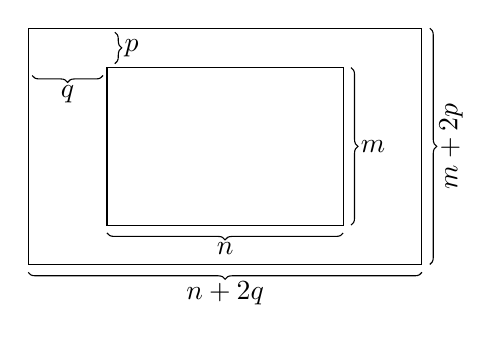
\begin{tikzpicture}
    \draw (0,0) rectangle (5,3);
    \draw (1,0.5) rectangle (4,2.5);
    \draw[decorate,decoration=brace] (5.1,3) -- node[midway,right]{\rotatebox{90}{$m+2p$}} (5.1,0);
    \draw[decorate,decoration=brace] (5,-0.1) -- node[midway,below]{$n+2q$} (0,-0.1);
    \draw[decorate,decoration=brace] (4.1,2.5) -- node[midway,right]{$m$} (4.1,0.5);
    \draw[decorate,decoration=brace] (4,0.4) -- node[midway,below]{$n$} (1,0.4);
    \draw[decorate,decoration=brace] (1.1,2.95) -- node[midway,right]{$p$} (1.1,2.55);
    \draw[decorate,decoration=brace] (0.95,2.4) -- node[midway,below]{$q$} (0.05,2.4);
  \end{tikzpicture}
\end{center}
Then, the output size will be
\[ \floor*{1+\frac{m+2p-a}{s}} \times \floor*{1+\frac{n+2q-b}{t}} \]
If we want the input and output to have the ``same'' size, set
\[ p = \ceil*{\frac{m(s-a)+a-s}{2}} \qq{and} q = \ceil*{\frac{n(t-1)+b-t}{2}} \]

\textrule{...one reading week later...}
\lecture{Feb 27}

Recall the convolution of $\X = \mqty[\Xmat*{x}{2}{2}]$
and $\W = \mqty[\Xmat*{w}{1}{1}]$:
\[
  \W \ast \X = \begin{bmatrix}
    w_{00}x_{00} + w_{01}x_{01} + w_{10}x_{10} + w_{11}x_{11}
     & w_{00}x_{01} + w_{01}x_{02} + w_{10}x_{11} + w_{11}x_{12} \\
    w_{00}x_{10} + w_{01}x_{11} + w_{10}x_{20} + w_{11}x_{21}
     & w_{00}x_{11} + w_{01}x_{12} + w_{10}x_{21} + w_{11}x_{22}
  \end{bmatrix}
\]
such that the vectorization is
\[
  \Vector(\W \ast \X) = \mqty[
  w_{00}x_{00} + w_{01}x_{01} + w_{10}x_{10} + w_{11}x_{11} \\
  w_{00}x_{01} + w_{01}x_{02} + w_{10}x_{11} + w_{11}x_{12} \\
  w_{00}x_{10} + w_{01}x_{11} + w_{10}x_{20} + w_{11}x_{21} \\
  w_{00}x_{11} + w_{01}x_{12} + w_{10}x_{21} + w_{11}x_{22}
  ]
\]
This is a linear transformation.
Therefore, we can design a \term{circulant matrix} $\W_\cir$
such that $\W_\cir\Vector(\X) = \Vector(\W \ast \X)$. Define
\[
  \W_\cir = \begin{bmatrix}
    w_{00} & w_{01} & 0      & w_{10} & w_{11} & 0      & 0      & 0      & 0      \\
    0      & w_{00} & w_{01} & 0      & w_{10} & w_{11} & 0      & 0      & 0      \\
    0      & 0      & 0      & w_{00} & w_{01} & 0      & w_{10} & w_{11} & 0      \\
    0      & 0      & 0      & 0      & w_{00} & w_{01} & 0      & w_{10} & w_{11}
  \end{bmatrix}
\]
and it is clear that $\W_\cir\Vector(\X) = \Vector(\W\ast\X)$.

Now, notice that we only need to learn $\abs{\W} = 4$ weights
instead of $\abs{\W_\cir} = 9 \times 4 = 36$ weights.

We can also down-sample the input size using \term{pooling}.
Just like convolution, we take a sliding window with some fixed size and stride
and apply a transformation.
Instead of the inner product, we can do \term[pooling!max]{max-pooling}
(take the max of the window) or \term[pooling!average]{average-pooling}
(take the mean of the window).
\term[pooling!global]{Global pooling} is where the window is the whole input,
so we output a single scalar.

\subsection*{Architecture Examples}

\paragraph{LeNet} Given an input of size $32^2$,
\begin{itemize}[nosep]
  \item Convolve with six $5^2$ kernels to 6 @ $28^2$
  \item Subsample down by half to 6 @ $14^2$
  \item Convolve with sixteen $5^2$ kernels to 16 @ $10^2$
  \item Subsample down by half to 16 @ $5^5$
  \item Fully connect to a 120-wide layer
  \item Fully connect to an 84-wide layer
  \item Gaussian connect to a 10-wide output
\end{itemize}

\paragraph{AlexNet} Given an input of size 3 @ $224 \times 224$:
\begin{itemize}[nosep]
  \item Convolve with 96 kernels to 96 @ $55 \times 55$
\end{itemize}

\lecture{Mar 5}
\section{Transformers}

TODO: up to slide 11

\begin{center}
  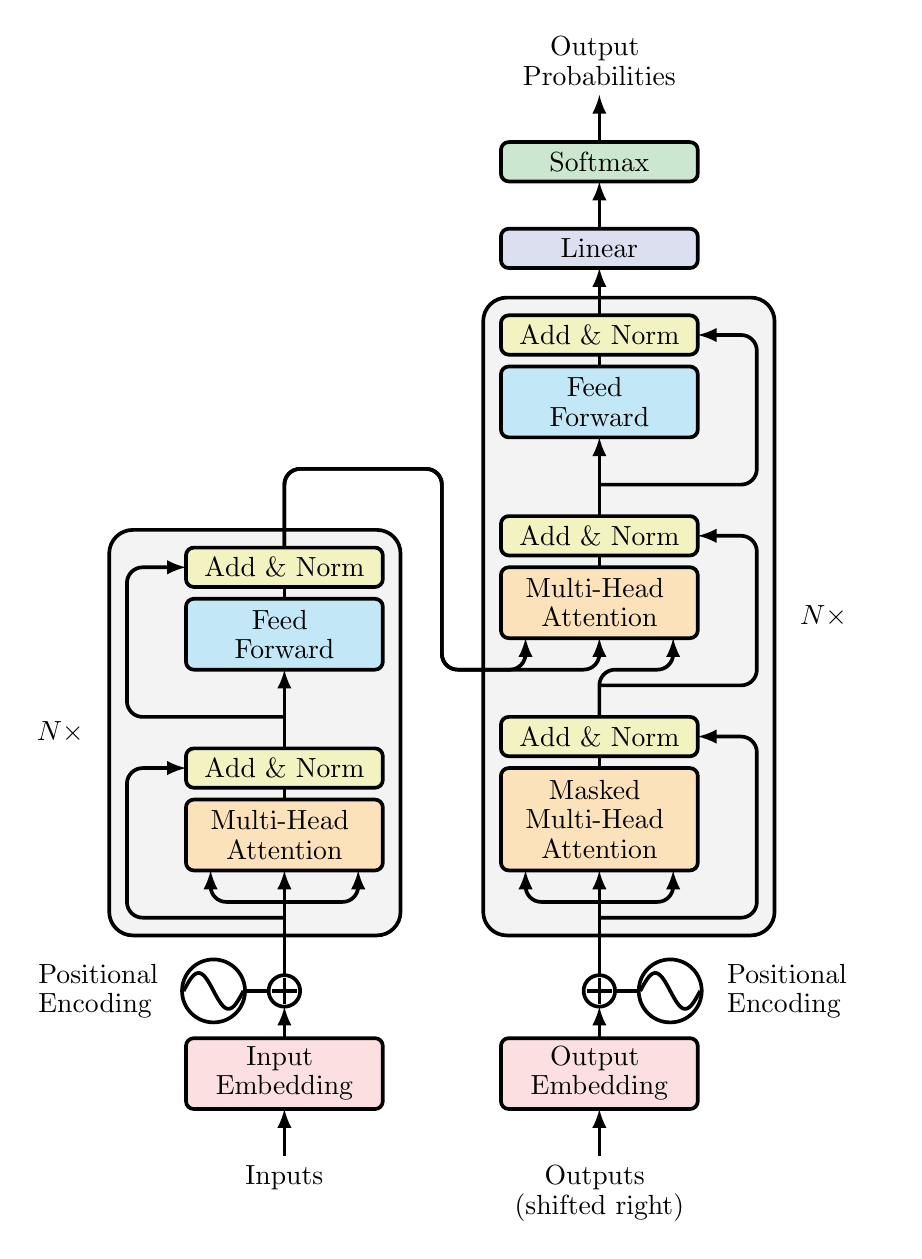
\begin{tikzpicture}
    \definecolor{emb_color}{RGB}{252,224,225}
    \definecolor{multi_head_attention_color}{RGB}{252,226,187}
    \definecolor{add_norm_color}{RGB}{242,243,193}
    \definecolor{ff_color}{RGB}{194,232,247}
    \definecolor{softmax_color}{RGB}{203,231,207}
    \definecolor{linear_color}{RGB}{220,223,240}
    \definecolor{gray_bbox_color}{RGB}{243,243,244}
    \draw[fill=gray_bbox_color, line width=0.046875cm, rounded corners=0.300000cm] (-0.975000, 6.455000) -- (2.725000, 6.455000) -- (2.725000, 1.305000) -- (-0.975000, 1.305000) -- cycle;
    \draw[fill=gray_bbox_color, line width=0.046875cm, rounded corners=0.300000cm] (3.775000, 9.405000) -- (7.475000, 9.405000) -- (7.475000, 1.305000) -- (3.775000, 1.305000) -- cycle;
    \draw[line width=0.046875cm, fill=emb_color, rounded corners=0.100000cm] (0.000000, 0.000000) -- (2.500000, 0.000000) -- (2.500000, -0.900000) -- (0.000000, -0.900000) -- cycle;
      \node[text width=2.500000cm, align=center] at (1.250000,-0.450000) {Input \vspace{-0.05cm} \linebreak Embedding};
    \draw[line width=0.046875cm, fill=emb_color, rounded corners=0.100000cm] (4.000000, 0.000000) -- (6.500000, 0.000000) -- (6.500000, -0.900000) -- (4.000000, -0.900000) -- cycle;
      \node[text width=2.500000cm, align=center] at (5.250000,-0.450000) {Output \vspace{-0.05cm} \linebreak Embedding};
    \draw[line width=0.046875cm, fill=add_norm_color, rounded corners=0.100000cm] (0.000000, 3.680000) -- (2.500000, 3.680000) -- (2.500000, 3.180000) -- (0.000000, 3.180000) -- cycle;
      \node[text width=2.500000cm, align=center] at (1.250000,3.430000) {Add \& Norm};
    \draw[line width=0.046875cm, fill=multi_head_attention_color, rounded corners=0.100000cm] (0.000000, 3.030000) -- (2.500000, 3.030000) -- (2.500000, 2.130000) -- (0.000000, 2.130000) -- cycle;
      \node[text width=2.500000cm, align=center] at (1.250000,2.580000) {Multi-Head \vspace{-0.05cm} \linebreak Attention};
    \draw[line width=0.046875cm] (1.250000, 3.030000) -- (1.250000, 3.180000);
    \draw[line width=0.046875cm, fill=add_norm_color, rounded corners=0.100000cm] (4.000000, 6.630000) -- (6.500000, 6.630000) -- (6.500000, 6.130000) -- (4.000000, 6.130000) -- cycle;
      \node[text width=2.500000cm, align=center] at (5.250000,6.380000) {Add \& Norm};
    \draw[line width=0.046875cm, fill=multi_head_attention_color, rounded corners=0.100000cm] (4.000000, 5.980000) -- (6.500000, 5.980000) -- (6.500000, 5.080000) -- (4.000000, 5.080000) -- cycle;
      \node[text width=2.500000cm, align=center] at (5.250000,5.530000) {Multi-Head \vspace{-0.05cm} \linebreak Attention};
    \draw[line width=0.046875cm] (5.250000, 5.980000) -- (5.250000, 6.130000);
    \draw[line width=0.046875cm, fill=add_norm_color, rounded corners=0.100000cm] (4.000000, 4.080000) -- (6.500000, 4.080000) -- (6.500000, 3.580000) -- (4.000000, 3.580000) -- cycle;
      \node[text width=2.500000cm, align=center] at (5.250000,3.830000) {Add \& Norm};
    \draw[line width=0.046875cm, fill=multi_head_attention_color, rounded corners=0.100000cm] (4.000000, 3.430000) -- (6.500000, 3.430000) -- (6.500000, 2.130000) -- (4.000000, 2.130000) -- cycle;
      \node[text width=2.500000cm, align=center] at (5.250000,2.780000) {Masked \vspace{-0.05cm} \linebreak Multi-Head \vspace{-0.05cm} \linebreak Attention};
    \draw[line width=0.046875cm] (5.250000, 3.430000) -- (5.250000, 3.580000);
    \draw[line width=0.046875cm, fill=add_norm_color, rounded corners=0.100000cm] (0.000000, 6.230000) -- (2.500000, 6.230000) -- (2.500000, 5.730000) -- (0.000000, 5.730000) -- cycle;
      \node[text width=2.500000cm, align=center] at (1.250000,5.980000) {Add \& Norm};
    \draw[line width=0.046875cm, fill=ff_color, rounded corners=0.100000cm] (0.000000, 5.580000) -- (2.500000, 5.580000) -- (2.500000, 4.680000) -- (0.000000, 4.680000) -- cycle;
      \node[text width=2.500000cm, align=center] at (1.250000,5.130000) {Feed \vspace{-0.05cm} \linebreak Forward};
    \draw[line width=0.046875cm] (1.250000, 5.580000) -- (1.250000, 5.730000);
    \draw[line width=0.046875cm, fill=add_norm_color, rounded corners=0.100000cm] (4.000000, 9.180000) -- (6.500000, 9.180000) -- (6.500000, 8.680000) -- (4.000000, 8.680000) -- cycle;
      \node[text width=2.500000cm, align=center] at (5.250000,8.930000) {Add \& Norm};
    \draw[line width=0.046875cm, fill=ff_color, rounded corners=0.100000cm] (4.000000, 8.530000) -- (6.500000, 8.530000) -- (6.500000, 7.630000) -- (4.000000, 7.630000) -- cycle;
      \node[text width=2.500000cm, align=center] at (5.250000,8.080000) {Feed \vspace{-0.05cm} \linebreak Forward};
    \draw[line width=0.046875cm] (5.250000, 8.530000) -- (5.250000, 8.680000);
    \draw[line width=0.046875cm, fill=linear_color, rounded corners=0.100000cm] (4.000000, 10.280000) -- (6.500000, 10.280000) -- (6.500000, 9.780000) -- (4.000000, 9.780000) -- cycle;
      \node[text width=2.500000cm, align=center] at (5.250000,10.030000) {Linear};
    \draw[line width=0.046875cm, fill=softmax_color, rounded corners=0.100000cm] (4.000000, 11.380000) -- (6.500000, 11.380000) -- (6.500000, 10.880000) -- (4.000000, 10.880000) -- cycle;
      \node[text width=2.500000cm, align=center] at (5.250000,11.130000) {Softmax};
    \draw[line width=0.046875cm] (1.250000, 0.600000) circle (0.200000);
    \draw[line width=0.046875cm] (1.410000, 0.600000) -- (1.090000, 0.600000);
    \draw[line width=0.046875cm] (1.250000, 0.760000) -- (1.250000, 0.440000);
    \draw[line width=0.046875cm] (5.250000, 0.600000) circle (0.200000);
    \draw[line width=0.046875cm] (5.410000, 0.600000) -- (5.090000, 0.600000);
    \draw[line width=0.046875cm] (5.250000, 0.760000) -- (5.250000, 0.440000);
    \draw[line width=0.046875cm] (0.350000, 0.600000) circle (0.400000);
    \draw[line width=0.046875cm] (-0.030000, 0.600000) -- (-0.014490, 0.629156) -- (0.001020, 0.657833) -- (0.016531, 0.685561) -- (0.032041, 0.711884) -- (0.047551, 0.736369) -- (0.063061, 0.758616) -- (0.078571, 0.778258) -- (0.094082, 0.794973) -- (0.109592, 0.808486) -- (0.125102, 0.818576) -- (0.140612, 0.825077) -- (0.156122, 0.827883) -- (0.171633, 0.826946) -- (0.187143, 0.822284) -- (0.202653, 0.813971) -- (0.218163, 0.802145) -- (0.233673, 0.786999) -- (0.249184, 0.768783) -- (0.264694, 0.747796) -- (0.280204, 0.724382) -- (0.295714, 0.698925) -- (0.311224, 0.671845) -- (0.326735, 0.643584) -- (0.342245, 0.614608) -- (0.357755, 0.585392) -- (0.373265, 0.556416) -- (0.388776, 0.528155) -- (0.404286, 0.501075) -- (0.419796, 0.475618) -- (0.435306, 0.452204) -- (0.450816, 0.431217) -- (0.466327, 0.413001) -- (0.481837, 0.397855) -- (0.497347, 0.386029) -- (0.512857, 0.377716) -- (0.528367, 0.373054) -- (0.543878, 0.372117) -- (0.559388, 0.374923) -- (0.574898, 0.381424) -- (0.590408, 0.391514) -- (0.605918, 0.405027) -- (0.621429, 0.421742) -- (0.636939, 0.441384) -- (0.652449, 0.463631) -- (0.667959, 0.488116) -- (0.683469, 0.514439) -- (0.698980, 0.542167) -- (0.714490, 0.570844) -- (0.730000, 0.600000);
    \draw[line width=0.046875cm] (6.150000, 0.600000) circle (0.400000);
    \draw[line width=0.046875cm] (5.770000, 0.600000) -- (5.785510, 0.629156) -- (5.801020, 0.657833) -- (5.816531, 0.685561) -- (5.832041, 0.711884) -- (5.847551, 0.736369) -- (5.863061, 0.758616) -- (5.878571, 0.778258) -- (5.894082, 0.794973) -- (5.909592, 0.808486) -- (5.925102, 0.818576) -- (5.940612, 0.825077) -- (5.956122, 0.827883) -- (5.971633, 0.826946) -- (5.987143, 0.822284) -- (6.002653, 0.813971) -- (6.018163, 0.802145) -- (6.033673, 0.786999) -- (6.049184, 0.768783) -- (6.064694, 0.747796) -- (6.080204, 0.724382) -- (6.095714, 0.698925) -- (6.111224, 0.671845) -- (6.126735, 0.643584) -- (6.142245, 0.614608) -- (6.157755, 0.585392) -- (6.173265, 0.556416) -- (6.188776, 0.528155) -- (6.204286, 0.501075) -- (6.219796, 0.475618) -- (6.235306, 0.452204) -- (6.250816, 0.431217) -- (6.266327, 0.413001) -- (6.281837, 0.397855) -- (6.297347, 0.386029) -- (6.312857, 0.377716) -- (6.328367, 0.373054) -- (6.343878, 0.372117) -- (6.359388, 0.374923) -- (6.374898, 0.381424) -- (6.390408, 0.391514) -- (6.405918, 0.405027) -- (6.421429, 0.421742) -- (6.436939, 0.441384) -- (6.452449, 0.463631) -- (6.467959, 0.488116) -- (6.483469, 0.514439) -- (6.498980, 0.542167) -- (6.514490, 0.570844) -- (6.530000, 0.600000);
    \draw[line width=0.046875cm, -latex] (1.250000, 3.680000) -- (1.250000, 4.680000);
    \draw[line width=0.046875cm, -latex] (5.250000, 6.630000) -- (5.250000, 7.630000);
    \draw[line width=0.046875cm, -latex] (5.250000, 9.180000) -- (5.250000, 9.780000);
    \draw[line width=0.046875cm, -latex] (5.250000, 10.280000) -- (5.250000, 10.880000);
    \draw[line width=0.046875cm, -latex] (1.250000, 0.000000) -- (1.250000, 0.400000);
    \draw[line width=0.046875cm, -latex] (1.250000, 0.800000) -- (1.250000, 2.130000);
    \draw[line width=0.046875cm, -latex] (5.250000, 0.800000) -- (5.250000, 2.130000);
    \draw[line width=0.046875cm, -latex] (5.250000, 0.000000) -- (5.250000, 0.400000);
    \draw[line width=0.046875cm] (0.750000, 0.600000) -- (1.050000, 0.600000);
    \draw[line width=0.046875cm] (5.450000, 0.600000) -- (5.750000, 0.600000);
    \draw[-latex, line width=0.046875cm, rounded corners=0.200000cm] (1.250000, 4.080000) -- (-0.750000, 4.080000) -- (-0.750000, 5.980000) -- (0.000000, 5.980000);
    \draw[-latex, line width=0.046875cm, rounded corners=0.200000cm] (1.250000, 1.530000) -- (-0.750000, 1.530000) -- (-0.750000, 3.430000) -- (0.000000, 3.430000);
    \draw[-latex, line width=0.046875cm, rounded corners=0.200000cm] (5.250000, 1.530000) -- (7.250000, 1.530000) -- (7.250000, 3.830000) -- (6.500000, 3.830000);
    \draw[-latex, line width=0.046875cm, rounded corners=0.200000cm] (5.250000, 4.480000) -- (7.250000, 4.480000) -- (7.250000, 6.380000) -- (6.500000, 6.380000);
    \draw[-latex, line width=0.046875cm, rounded corners=0.200000cm] (5.250000, 7.030000) -- (7.250000, 7.030000) -- (7.250000, 8.930000) -- (6.500000, 8.930000);
    \draw[-latex, line width=0.046875cm, rounded corners=0.200000cm] (1.250000, 1.730000) -- (0.312500, 1.730000) -- (0.312500, 2.130000);
    \draw[-latex, line width=0.046875cm, rounded corners=0.200000cm] (1.250000, 1.730000) -- (2.187500, 1.730000) -- (2.187500, 2.130000);
    \draw[-latex, line width=0.046875cm, rounded corners=0.200000cm] (5.250000, 1.730000) -- (4.312500, 1.730000) -- (4.312500, 2.130000);
    \draw[-latex, line width=0.046875cm, rounded corners=0.200000cm] (5.250000, 1.730000) -- (6.187500, 1.730000) -- (6.187500, 2.130000);
    \draw[-latex, line width=0.046875cm, rounded corners=0.200000cm] (1.250000, 6.230000) -- (1.250000, 7.230000) -- (3.250000, 7.230000) -- (3.250000, 4.680000) -- (4.312500, 4.680000) -- (4.312500, 5.080000);
    \draw[-latex, line width=0.046875cm, rounded corners=0.200000cm] (1.250000, 6.230000) -- (1.250000, 7.230000) -- (3.250000, 7.230000) -- (3.250000, 4.680000) -- (5.250000, 4.680000) -- (5.250000, 5.080000);
    \draw[-latex, line width=0.046875cm, rounded corners=0.200000cm] (5.250000, 4.080000) -- (5.250000, 4.680000) -- (6.187500, 4.680000) -- (6.187500, 5.080000);
    \draw[line width=0.046875cm, -latex] (1.250000, -1.500000) -- (1.250000, -0.900000);
    \draw[line width=0.046875cm, -latex] (5.250000, -1.500000) -- (5.250000, -0.900000);
    \draw[line width=0.046875cm, -latex] (5.250000, 11.380000) -- (5.250000, 11.980000);
      \node[text width=2.500000cm, anchor=north, align=center] at (1.250000,-1.500000) {Inputs};
      \node[text width=2.500000cm, anchor=north, align=center] at (5.250000,-1.500000) {Outputs \vspace{-0.05cm} \linebreak (shifted right)};
      \node[text width=2.500000cm, anchor=south, align=center] at (5.250000,11.980000) {Output \vspace{-0.05cm} \linebreak Probabilities};
      \node[anchor=east] at (-1.175000,3.880000) {$N\times$};
      \node[anchor=west] at (7.675000,5.355000) {$N\times$};
      \node[text width=2.000000cm, anchor=east] at (0.250000,0.600000) {Positional \vspace{-0.05cm} \linebreak Encoding};
      \node[text width=2.000000cm, anchor=west] at (6.750000,0.600000) {Positional \vspace{-0.05cm} \linebreak Encoding};
  \end{tikzpicture}
\end{center}

Our goal is given a sequence of tokens (the prompt) $X = (\x_1,\dotsc,\x_n)$,
to find a sequence $Y = (\vb y_1,\dotsc,\vb y_m)$ such that the maximum likelihood
\[ \argmax_{Y} p(\vb y_1,\dotsc,\vb y_m \mid \x_1,\dotsc,\x_n) \]
is achieved.
We use an \term{auto-regressive} model where we greedily take
\[ \argmax_{\vb y_k} p(\vb y_k \mid \x_1,\dotsc,\x_n,\vb y_1,\dotsc,\vb y_{k-1}) \]
i.e., one token at a time.
Note that $m$ is not pre-defined; we keep generating until we reach the [END] token.

At each step, we input the \textcolor{Red}{\textbf{embeddings}} of the prompt and the partially generated text.
The text is converted to tokens, which are the smallest elements the model can understand.
Then, the tokens are embedded in a high-dimensional vector space (typically, $d=512$).
The embedding should map similar words to similar locations.

The output of the prompt embedding is $X = [\x_1,\dotsc,\x_n] \in \R^{n \times d}$
and the auto-regressive outputs $[\vb y_1,\dotsc,\vb y_k] \in \R^{k \times d}$

Since word order matters, we also add a \textbf{positional encoding}.
We define the matrix $W^p \in \R^{n \times d}$ as
\[ W^p_{t,2i} = \sin(t/10000^{2i/d})\qc W^p_{t,2i+1} = \cos(t/10000^{2i/d})\qc i = 0,\dotsc,\tfrac{d}{2}-1 \]
This is a fixed part of the model, and we simply add $W^p$ to $X$.
The auto-regressive output is also similarly positionally encoded.

These are then sent to \textcolor{Orange}{\textbf{attention layers}}.

The Attention function has an input value $V \in \R^{n \times d}$,
a key $K \in \R^{n \times d}$, and a query $Q \in \R^{m \times d}$.
It outputs an $\R^{m \times d}$ matrix.

Recall the softmax function (\cref{eq:softmax}) as applied to vectors:
\[ \softmax(\z) = \qty[\frac{\exp(z_1)}{\sum_i \exp(z_i)},\dotsc,\frac{\exp(z_n)}{\sum_i \exp(z_n)}] \]
Then, writing $\v_i\trans$, $\k_i\trans$, and $\q_i\trans$ as the rows of $V$, $K$, and $Q$:
\begin{align*}
    & \operatorname{Attention}(V,K,Q)                                                                                                                                                                                                                                                                                                                              \\
  = & \softmax\qty(\frac{QK\trans}{\sqrt d})V                                                                                                                                                                                                                                                                                                                      \\
  = & \begin{bmatrix}
        \softmax\qty(\frac{\ip{\q_1}{\k_1}}{\sqrt d}) & \softmax\qty(\frac{\ip{\q_1}{\k_2}}{\sqrt d}) & \cdots & \softmax\qty(\frac{\ip{\q_1}{\k_n}}{\sqrt d}) \\
        \softmax\qty(\frac{\ip{\q_2}{\k_1}}{\sqrt d}) & \softmax\qty(\frac{\ip{\q_2}{\k_2}}{\sqrt d}) & \cdots & \softmax\qty(\frac{\ip{\q_2}{\k_n}}{\sqrt d}) \\
        \vdots                                        & \vdots                                        & \ddots & \vdots                                        \\
        \softmax\qty(\frac{\ip{\q_m}{\k_1}}{\sqrt d}) & \softmax\qty(\frac{\ip{\q_m}{\k_2}}{\sqrt d}) & \cdots & \softmax\qty(\frac{\ip{\q_m}{\k_n}}{\sqrt d})
      \end{bmatrix}V                               \\
  = & \begin{bmatrix}
        \softmax\qty(\frac{\ip{\q_1}{\k_1}}{\sqrt d})\v_1\trans + \softmax\qty(\frac{\ip{\q_1}{\k_2}}{\sqrt d})\v_2\trans + \dotsb + \softmax\qty(\frac{\ip{\q_1}{\k_n}}{\sqrt d})\v_n\trans \\
        \softmax\qty(\frac{\ip{\q_2}{\k_1}}{\sqrt d})\v_1\trans + \softmax\qty(\frac{\ip{\q_2}{\k_2}}{\sqrt d})\v_2\trans + \dotsb + \softmax\qty(\frac{\ip{\q_2}{\k_n}}{\sqrt d})\v_n\trans \\
        \vdots                                                                                                                                                                               \\
        \softmax\qty(\frac{\ip{\q_m}{\k_1}}{\sqrt d})\v_1\trans + \softmax\qty(\frac{\ip{\q_m}{\k_2}}{\sqrt d})\v_2\trans + \dotsb + \softmax\qty(\frac{\ip{\q_m}{\k_n}}{\sqrt d})\v_n\trans
      \end{bmatrix} \in \R^{m \times d}
\end{align*}
Each output ``value'' (i.e., row) here is a convex combination of the rows of $V$.

In the self-attention case, $Q = K = V = $ whatever the input is.

So far, there are no learnable parameters.
To add learnable parameters, we do a linear layer with each of $V$, $K$, and $Q$.
That is, $W^q_i,W^k_i,W^v_i \in \R^{512 \times 64}$ can be learnable linear layers
such that $\operatorname{Attention}_i = \softmax\qty(\frac{QW^q_i(KW^k_i)\trans}{\sqrt{d}})VW^v_i$.

Each of these $i = 1,\dotsc,h$ triplets is called a head.
Typically $h = 8$.
A multi-head attention layer concatenates each $\operatorname{Attention}_i$
and sends that through a final learnable linear layer.

A masked attention layer just ignores future tokens $\vb y_k,\dotsc,\vb y_m$ during training.

The \textcolor{Cerulean}{\textbf{feed forward layers}} are just two-layer MLPs
with ReLU activation:
\[ \max(0,\x\trans W_1 + \vb b_1)W_2 + \vb b_2 \]
where $W_1 \in \R^{d \times 4d}$ and $W_2 \in \R^{4d \times d}$.
They also have \textcolor{Dandelion}{\textbf{residual connections}}
and \textcolor{Dandelion}{\textbf{layer normalization}}.

\paragraph{Summary}
There are three tunable hyperparameters: layers $N = 6$,
output dimensions $d = 512$, and heads $h = 8$.

The cross-attention module has $V = K = $ encoder and $Q = $ decoder.
The other attention modules are self-attentive, so $V = K = Q$.

We train by minimizing the log-loss between true next words and predicted next words
\[ \min_W \hat{\E}[-\ip{Y}{\log\hat Y}] \]
where $Y = [\vb y_1,\dotsc,\vb y_l]$ is the one-hot output sequence
and $\hat Y = [\vb{\hat{y}}_1,\dotsc,\vb{\hat{y}}_l]$ are the predicted probabilities.

\chapter{Modern Machine Learning}

\section{Large Language Models}

TOOD: up to slide 9

\subsection*{Generative Pre-Training (GPT-1)}

GPT-1 is an open-source 12-layer decoder with 110M parameters.
It is pre-trained unsupervised on next-word prediction.
Then, fine-tuning is done on task-dependent architecture, i.e.,
there are specific

\subsection*{Bidirectional Encoder Representations from Transformers (BERT)}

BERT is an encoder-only model.
It also has a pre-training phase and fine-tuning phase.

In the pre-training phase,
the encoder is given masked sentences and is trained to generate the missing tokens
(Masked LM; task A).
Training on task A performs better than training on the left-to-right prediction task.
The model is also trained on next-sentence prediction (NSP; task B),
where it binary classifies whether two sentences follow or are unrelated.

$\text{BERT}_\text{BASE}$ has a similar number of parameters (110M) to GPT-1,
but performs better.
$\text{BERT}_\text{LARGE}$ (340M) performs better than both.

RoBERTa (Robustly Optimized BERT Approach) is just a larger BERT model
with bigger batches and more data.
It was also only trained on the Masked LM objective,
but with longer sequences.

Sentence-BERT/RoBERTa trains the similarity task using two encoders
(one for each sentence) and saves represented encodings.
This saves a lot of inference time.

\subsection*{GPT-2 through 4}

Basically the only thing done is make the model larger.

GPT-2 introduced a new dataset called WebText.
The 1.5B-parameter model is around $10\times$ larger than GPT-1,
and is trained in the same way.
It is about on par with BERT on finetuning tasks.
It is also the most recent OpenAI model to be open-sourced.
However, it is very good at zero-shot learning.
This means we no longer need task-dependent architecture.

GPT-3 is trained exactly the same as GPT and GPT-2,
but $100\times$ larger (175B parameters).
At around the 100B-parameter level,
we start to see emergent properties of in-context learning (zero-/few-shot prompts)
and chain-of-thought (either one-shot or ``let's do this step-by-step'').
However, raw language models do not answer questions or behave in a chat-like way.
For example, asking a quesiton to GPT-3 will result in a list of similar questions.

GPT-3.5 (InstructGPT) uses Reinforcement Learning from Human Feedback (RLHF).
In RLHF, the agent uses a policy function (LLM)
to take actions (outputs) given a state (prompt),
and is returned a reward and new state based on the environment (another LLM):
\begin{enumerate}
  \item Collect demonstration data, and train a supervised policy:
        train by overfitting GPT-3 to human-written desired outputs
        (the SFT model).
  \item Collect comparison data, and train a reward model:
        train a new reward model (RM) using human rankings of outputs.
        We use pair-wise comparison logistic loss
        \[ \operatorname{loss}(\theta) = -\E_{(x,y_w,y_l)}[\log(\sigma(r_\theta(x,y_w) - r(x,y_l)))] \]
        for a prompt $x$ and preferred output $r_\theta(x,y_w) \gg r_\theta(x,y_l)$.
        This trains a real-valued function $r_\theta$ so ChatGPT knows
        how much better $y_w$ is than $y_l$ without the unknown human element.
  \item Optimize a policy against the reward model using reinforcement learning:
        update the SFT model using the RM model using proximal policy optimization (PPO):
        \[
          \max_\phi \E_{(x,y)} [
          \underbrace{r_\theta(x,y)}_{\text{RM reward}}
          - \beta\underbrace{\log(\pi_\phi^{\text{RL}}(y \mid x) / \pi^{\text{SFT}(y \mid x)})}_{\text{model is close to SFT}}
          ] + \gamma\underbrace{\E[\log(\pi_\phi^{\text{RL}}(x))]}_{\text{pretraining loss}}
        \]
\end{enumerate}
In general, GPT $\ll$ prompted GPT $\ll$ SFT $\ll$ PPO $<$ PPO with pretraining mix.
PPO-ptx is the base model for ChatGPT-3.5 and GitHub Copilot.

GPT-4 allows combined multimodal image/text input.
The paper says nothing so nobody knows how it works.

\section{Generative Adversarial Networks}

\lecture{Mar 12}

Suppose we are given training data $\{\x_i\} \sim q(\x)$, i.e.,
with \term{data density} $q(\x)$.
Recall that $q(\x)$ is a distribution if $\int_{-\infty}^\infty q(\x) \dd{\x} = 1$
and $q(\x) \geq 0$.

We will develop a \term{model density} $p_{\vth}(\x)$
paramaterized by $\vth$.
We will find $\vth$ by minimizing some ``distance'' between $q$ and $p_{\vth}$.
In particular, we will minimize the KL divergence
\begin{align*}
  \KL(q \parallel p_{\vth})
   & := \int q(\x)\log\frac{q(\x)}{p_{\vth}(\x)}        \\
   & \equiv \int -\log p_{\vth}(\x) \cdot q(\x) \dd{\x} \\
   & = \E_{\x \sim q(\x)}[-\log p_{\vth}(\x)]           \\
   & \approx -\frac1n \sum_{i=1}^n\log p_{\vth}(\x_i)
\end{align*}
Then, we will use $p_{\vth}(\x)$ to generate new data $\rv X \sim p_{\vth}(\x)$.

However, we do not have a closed-form way to calculate $p_{\vth}$.
Suppose that we want $p(\x)$ to be a $d$-variate Gaussian with means $\vmu \in \R^d$
and covariance matrix $S \in \R^{d \times d}$:
\[ p(\x) = (2\pi)^{d/2}[\det(S)]^{-1/2}\exp[-\frac12(\x-\vmu)\trans S^{-1}(\x-\vmu)] \]
To draw from $p(\x)$, start by drawing $\vb n \sim \normal(\vb 0, \id)$.
Then, we write $\x = L\vb n + \vmu$ where $LL\trans = S$
(the \term{Chloesky decompostion} of $S$),
so that we have
\begin{align*}
  \E[\x]                       & = E[L\vb n + \vmu] = \vmu                                  \\
  \E[(\x-\vmu)(\x-\vmu)\trans] & = L\cdot\E[\vb n \vb n\trans] \cdot L\trans = LL\trans = S
\end{align*}
and $p(\x) = \normal(\vmu,S)$, as desired.

We will simply replace the function $L\vb n + \vmu$ with a neural network.

\begin{theorem}[representation through push-forward]\label{thm:push}
  Let $r$ be any continuous distribution on $\R^h$.
  Then, for any distribution $p$ on $\R^d$, there exist \term{push-forward maps}
  $\T : \R^h \toto \R^d$ such that
  \[ \rv Z \sim r \implies \T(\rv Z) \sim p \]
\end{theorem}

This does not hold if $r$ has a delta mass at any point.
\WLOG, we take $r$ to be standard Gaussian noise.

We will learn $\T$ using a neural network.
In general, $\T$ is not unique, so we can optionally add restrictions to force uniqueness.
It can be a really weird set of mappings if $h \ll d$.

Now, we are able to generate new data $\rv X \sim p_{\vth} = \T_{\vth}(\rv Z)$
where $\rv Z \sim \normal(\vb 0,\id)$.
This means that we can easily \emph{draw from $p_{\vth}$}
but we cannot \emph{write the density function}.

We're stuck in a catch-22: we need the density to find the loss and train,
and we need the final trained $\T$ to draw.
Consider again the KL divergence:
\begin{align*}
  \KL(q \parallel p_{\vth}) & = \int \log\frac{q(\x)}{p_{\vth}(\x)} \dd{\x}
  \equiv \int \underbrace{\frac{q(\x)}{p_{\vth}(\x)}\qty[\log\frac{q(\x)}{p_{\vth}(\x)}-1]}_{f(\frac{q(\x)}{p_{\vth}(\x)})} \cdot p_{\vth}(\x) \dd{\x} \nr{eq:kl2}
\end{align*}
which we have rewritten as a function $f : \R_+ \to \R$, $f(t) = t\log t - t + 1$ of the ratio.

This is convex, because $\dv[2]{t} f(t) = \dv{t} \log t = \frac1t > 0$.

\begin{defn}[Fenchel conjugate]
  The conjugate of any function $f$ is the convex function $f^*(s) := \max_t st - f(t)$.

  Then, if $f$ is convex and continuous, then $f = f^{**}$.
\end{defn}

Since our $f$ is convex and continuous, let's try writing $f$ as $f^{**}$. First,
\begin{align*}
  f^*(s) & = [\max_t st - f(t)]            \\
         & = \max_t [st - t\log t + t - 1] \\
  \intertext{Then, setting the derivative to 0, we get $s = \log t$, i.e., $t = \exp s$, so}
  f^*(s) & = \exp s - 1
\end{align*}
This gives us
\[ f(t) = \max_s [st - f^*(s)] = \max_s [st - \exp s + 1] \]
Revisiting \cref{eq:kl2}, we can replace $f$ by $f^{**}$:
\begin{align*}
  \KL(q \parallel p_{\vth})
   & \equiv \int \qty[f\qty(\frac{q(\x)}{p_{\vth}(\x)})-1]\cdot p_{\vth}(\x) \dd{\x}                                                     \\
   & = \int \qty[\max_s s\frac{q(\x)}{p_{\vth}(\x)} - \exp s] \cdot p_{\vth}(\x) \dd{\x}                                                 \\
   & = \int \qty[\max_s sq(\x) - \exp(s)p_{\vth}(\x)] \dd{\x} \tag{$p_{\vth}(\x)$ has no $s$-dependence}                                 \\
   & = \max_{S : \R^d \to \R} \int [S(\x)q(\x) - \exp(S(\x))p_{\vth}(\x)] \dd{\x} \tag{$s$ is paramaterized by $\x$}                     \\
   & \approx \max_{S : \R^d \to \R} \frac1n\sum_{i=1}^n S(\x_i) - \frac1m \sum_{j=1}^m \exp[S(\T_{\vth}(\z_j))] \tag{by \cref{thm:push}}
\end{align*}
where $\x_i \sim q(\x)$ and $\z_j \sim \normal(\vb 0, \id)$.
We write this as one line:
\begin{equation}
  \min_{\vth} \KL(q \parallel p_{\vth})
  \approx \min_{\vth} \max_{\vphi} \frac1n\sum_{i=1}^n S_{\vphi}(\x_i) - \frac1m \sum_{j=1}^m \exp[S_{\vphi}(T_{\vth}(\z_j))]
\end{equation}
for a \term{generator} $\T_{\vth}$ which maps latent noise $\z$ to observation $\x$,
and a \term{discriminator} $S_{\vphi}$ which distinguishes data $\x$ from generation $\T_{\vth}(\z)$.

Both are neural networks paramaterized by weights $\vth$ and $\vphi$, respectively.

This ends up being a minimax game between the generator and discriminator.
At the equilibrium, the generator can make data and the discriminator cannot distinguish.

In reality, we do not use KL divergence, but instead JS divergence
\begin{align*}
  JS(q \parallel p_{\vth})
   & := \KL(q \parallel \tfrac{q+p_{\vth}}{2}) + \KL(q \parallel \tfrac{q+p_{\vth}}{2})                                                                                   \\
   & = \int q(\x) \log\frac{2q(\x)}{q(\x)+p_{\vth}(\x)} + p_{\vth}(\x)\log\frac{2p_{\vth}(\x)}{q(\x)+p_{\vth}(\x)} \dd{\x}                                                \\
   & = \int \qty[\frac{q(\x)}{p_{\vth}(\x)}\log\frac{q(\x)/p_{\vth}(\x)}{q(\x)/p_{\vth}(\x) + 1} + \log\frac{1}{q(\x)/p_{\vth}(\x)+1} + \log 4]\cdot p_{\vth}(\x) \dd{\x} \\
   & = \int f\qty(\tfrac{q(\x)}{p_{\vth}(\x)}) \cdot p_{\vth}(\x) \dd{\x}
\end{align*}
where $f(t) = t\log t - (t+1)\log(t+1) + \log4$ is convex.
Then, $f^*(t) = -\log(1-\exp s) - \log 4$.

If we do the same transformation, we can approximate
\[
  \min_{\vth} JS(q \parallel p_{\vth})
  \approx \min_{\vth} \max_{\vphi} \frac1n\sum_{i=1}^n S_{\vphi}(\x_i) - \frac1m \sum_{j=1}^m \log[1-\exp S_{\vphi}(T_{\vth}(\z_j))] - \log 4
\]

\begin{xca}
  Verify that this is true.
\end{xca}

Why do we use JS divergence? After the same transformations,
we can apply the change of variable $S_{\vphi} \gets \log S_{\vphi}$:
\[
  \min_{\vth} JS(q \parallel p_{\vth})
  \approx \min_{\vth} \max_{\vphi} \frac1n\sum_{i=1}^n \log S_{\vphi}(\x_i) - \frac1m \sum_{j=1}^m \log[1-S_{\vphi}(T_{\vth}(\z_j))]
\]
Let $\y(\x) = [\text{$\x$ is real data}]$.
Let $\mathfrak{p}_1(\x) = S_{\phi}(\x)$ be the (learnable) probability of $\x$ being real,
and $\mathfrak{p}_0 = 1 - \mathfrak{p}_1$. Then, we have:
\[ \min_{\vth} \max_{\vphi} \hat{\E}_{\rv X}\log \mathfrak{p}_{\y(\rv X)} \]
which is just the logistic regression (\cref{ch:lr}), which we know well.

\lecture{$\pi$}
In fact, we can prove that if we pick any strictly convex function $f : \R_+ \to \R$
with normalization $f(1) = 0$, then we can define an $f$-divergence $\bb D_f$
such that $\bb D_f (q \parallel p) \geq 0$ iff $p = q$ and we can maximize
\begin{align*}
  \min_{\vth} \bb D_f(q \parallel p)                                                                                            \\
   & := \min_{\vth}\int f(\tfrac{q(\x)}{p_{\vth}(\x)}) p_{\vth}(\x) \dd{\x}                                                     \\
   & \approx \min_{\vth}\max_{\vphi} \frac1n \sum_{n=1}^n S_{\vphi}(\x_i) - \frac1m \sum_{j=1}^m f^*[S_{\vphi}(T_{\vth}(\z_j))]
\end{align*}

MMD-GAN: Use a reproducing kernel to introduce non-linearity to the discriminator.

Wasserstein GAN: Suppose that the discriminator $S$ is Lipschitz continuous.
Then, paramaterize $S$ as a neural network and optimize over all Lipschitz functions.

\section{Flows}

Instead of minimizing distance, we can try to explicitly learn $q$ as a function of $p_{\vth}$.

\begin{remark}
  Let $\T : \R^d \toto \R^d$.
  Write $\nabla\T = (\nabla T_1,\dotsc,\nabla T_d) : \R^d \toto \R^d \otimes \R^d$.

  Since $\T\circ\T^{-1} = \id$,
  then $\nabla\T(\T^{-1})\cdot\nabla\T^{-1} = \id$ by the chain rule.
\end{remark}

\begin{theorem}[push-forward as change-of-variable]
  Let $r$ be any continuous distribution on $\R^d$.
  If the push-forward map $\T : \R^d \to \R^d$ is invertible,
  then the density of $\rv X := \T(\rv Z)$ is
  \[
    p(\x) = r(\T^{-1}\x) \cdot \abs{\det(\nabla\T^{-1}\x)}
    = \frac{r(\T^{-1}\x)}{\abs{\det(\nabla\T(\T^{-1}\x))}}
  \]
\end{theorem}
\begin{prf}[sketchy. physicisty. gross.]
  Roughly speaking, this means that $p(\x) \dd{\x} = r(\z) \dd{\z}$, i.e.,
  the ``mass'' of the distribution is preserved.

  We can ``rearrange'' to write $p(\x) = \dv{\z}{\x}r(\z)$.
  By definition, $r(\z)$ will be $\T^{-1}\x$.
  The ``derivative'' $\dv{\z}{\x}$ will be $\nabla \T^{-1}\x$,
  but we need it as a scalar, so it pops out as $\abs{\det(\nabla\T^{-1}\x)}$.
\end{prf}

\begin{notation}
  Write $p = \T_\#r$ to notate the above definition for $p(\x)$.
\end{notation}

Now, suppose we plug this into the KL-divergence:
\[
  \min_{\T} \KL(q \parallel \T_\#r) \approx
  \max_{\T} \frac1n\sum_{i=1}^n\qty[\log r(\T^{-1}\x_i) - \log\abs{\det \nabla\T(\T^{-1}\x_i)}]
\]
and learn $\T$. However, this is pretty hard to do,
since we have to express the inverse of $\T$ and the determinant of the $d \times d$ gradient matrix of $\T$.

Instead, we can learn the inverse during training:
\[
  \max_{\vb S = \T^{-1}} \frac1n\sum_{i=1}^n\qty[\log r(\vb S\x_i) - \log\abs{\det \nabla\vb S\x_i}]
\]
but then we need to invert $\vb S$ to recover $\T$ for sampling.
These both suck.
We prefer paying the cost during training, since that is a one-time cost.

We can be extremely clever with our construction of $\T$ to try to avoid this.
Suppose that we construct $\T$ as a \term{triangular map}
such that $\nabla \T(\z)$ is lower triangular, i.e.,
$T_i$ depends only on the first $i$ inputs.
This is very natural, since saying the $i$\xth output can only look at
elements ``before it'' sounds like causality.

Also, suppose that $\T$ is increasing on the $j$\xth output for the $j$\xth input,
i.e., the diagonal of $\nabla\T(\z)$ is positive.

Now, since $\nabla\T$ is triangular,
it's cheap to calculate the determinant as the product of the diagonal.
We went from an $\order{d^3}$ operation to $\order{d}$, which is way better.

Since $T_i$ only depends on $x_i$ and (already solved) previous elements,
and it is increasing w.r.t. $x_i$, we can use binary search to invert each element.
Bisections are basically free, so this is also $\order{d}$.

Therefore, increasing triangular maps work very well for our purposes.
We can also prove that they work.

\begin{theorem}[uniqueness for increasing triangular maps]
  For any two densities $r$ and $p$ on $\R^d$,
  there exists a unique (up to permutation) increasing triangular map $\T$
  such that $p = \T_\#r$.
\end{theorem}

If we fix $r$ as noise, this means that
any property of the probabilistic density $p$
is fully captured in the deterministic map $\T$!

This means that we can optimize
\[
  \min_{\T} \KL(q \parallel T_\#r) \approx
  \max_{\T} \frac1n\sum_{i=1}^n\qty[\log r(\T^{-1}\x_i) - \sum_{j=1}^d\log\nabla_jT_j(\T^{-1}\x_i)]
\]
where it only takes $\order{d}$ time for each training step.
There are a lot of models that are just this in disguise.

Autoregressive models (like GPT) calculate
$p_1(x_1), p_2(x_2 \mid x_1), \dotsc, p_j(x_j \mid x_{<j})$
which will be a triangular map.

If we suppose that each one of these distributions are Gaussian,
we get an increasing triangular map.
However, nested Gaussians can only produce Gaussians.
To add in non-normality, permute the entries randomly after each layer (masked AR flows).

\lecture{Mar 19}
The real-NVP model works by splitting the data into $\z_1=\{z_1,\dotsc,z_{l-1}\}$
and $\z_2 = \{z_l,\dots,z_d\}$.
The first segment is just copied $\x_1 = \z_1$
but the second part is fed through a map
\[
  T_j(z_j; z_1,\dotsc,z_{l-1}) = \exp(\alpha_j(z_1,\dotsc,z_{l-1})\cdot\symbf1_{j\geq l}) \cdot z_j + \mu_j(z_1,\dotsc,z_{l-1})\cdot\symbf1_{j\geq l}
\]
where $T$ ends up as a triangular map.

If we replace the linear wrapping of Gaussians with neural networks,
we end up with a neural AR flow.

If we use a polynomial, this is a sum-of-squares model.

\begin{theorem}[inverse sampling]
  Let $\rv Z \sim U(0,1)$, $F$ be the cdf of $\rv X$, and $Q = F^{-1}$ be the quantile function of $\rv X$.
  Then, $Q(\rv Z) \sim F$.
\end{theorem}

The function $\vb T : \R^d \to \R^d$ pushes the noise $\rv Z$ forward to observation $\rv X$.
The inverse map $\vb T^{-1}$ pulls observations $\rv X$ back to noise $\rv Z$.

This lets us generate anything from a uniform random generator.
In particular, we can send noise to uniform, and then uniform to data.

\section{Diffusion Models}

Suppose we had infinite layers of the masked AR flows. Recall that we set
\[
  \x_{t+1} \approx \x_t + \eta_t \cdot \f_t(\x_t) =: \T_t(\x_t)
\]
In the continuous case, we can express this as an ODE
\[ \dd{\x_{t+1}} = \f_t(\x_t)\dd{t} \]
for doing theory. In practice, we use the discrete form,
since that's all we can do with real computers.

Suppose each $\x_t \sim p_t$. In particular, since $\x_{t+1} \sim p_{t+1}$, we can write
\begin{align*}
  \log p_{t+1}(\x_{t+1})
   & = \log p_t(\x_t) - \log\abs{\det\partial_{\x}\T_t(\x_t)}                \\
   & = \log p_t(\x_t) - \log\abs{\det[\id + \eta_t \cdot \partial_{\x}\f_t(\x_t)]} \\
   & \approx \log p_t(\x_t) - \eta_t \cdot \ip{\partial_{\x}}{\f_t(\x_t)}
\end{align*}
where we make the last approximation by Taylor expansion of $\log(x)$ at $x=1$.
Then, in the continuous limit as $\eta_t \to 0$,
we can conclude that
\[ \dv{\log p_t(\x_t)}{t} = -\ip{\partial_{\x}}{\f_t(\x_t)} \]
From this, we can develop an MLE and learn.

We define the forward process as going from data to noise following
\[ \dd{\x} = \f_t(\x,t)\dd{t} + g(t) \dd{\w} \]
and the reverse process using stochastic gradient ascent following
\[ \dd{\x} = \qty[\f(\x,t) - g^2(t)\nabla_{\x}\log p_t(\x)] \dd{t} + g(t) \dd{\overline{\w}} \]
for some \term{score function} $\nabla_{\x}\log p_t(\x)$.
The score function is the only thing we need to learn,
because $\f$ is chosen (the forward process) and $g$ is also chosen (the variance of the noise).
We will use the forward process to learn the score function,
just like how the discriminator in GANs is used during training and discarded.

To develop the addition of noise, we can write a stochastic differential equation
\[ \dd{\x_{t+1}} = \f_t(\x_t) \dd{t} + G_t(\x_t) \dd{\n_t} \]
where $\n_t \sim \normal(0,1)$ (??) which we can discretize as
\[ \x_{t+1} \approx \x_t + \eta_t \cdot \f_t(\x_t) + \g_t(\x_t) \]
where $\g_t(\x_t) \sim \normal(\symbf0,\eta_t^2G_t(\x_t)G_t(\x_t)\trans)$.

Trivially, an ODE is just an SDE with $G_t \equiv \symbf0$.
Conversely, any SDE is equivalent to an ODE by replacing $\f_t$
with $\f_t - \frac12(G_tG_t\trans)\partial_{\x} - \frac12(G_tG_t\trans)\partial_{\x}\log p_t$.
Since we typically pick $G_t$ to have no $\x$-dependence,
the only important term here is the score function.

We can write the reverse-time SDE as
\[ \dd{\overline{\x_{t+1}}} = \overline{\f_t}(\overline{\x_t}) \dd{t} + G_t(\overline{\x_t}) \dd{\overline{\n_t}} \]
where $\overline{\f_t} = -\f_t + (G_tG_t\trans)\partial_{\x} + (G_tG_t\trans)\partial_{\x}\log p_t$
and time flows backwards for $\overline{\text{barred}}$ variables.

% \chapter{Trustworthy Machine Learning}

\pagebreak
\phantomsection\addcontentsline{toc}{chapter}{Back Matter}
\renewcommand{\listtheoremname}{List of Named Results}
\phantomsection\addcontentsline{toc}{section}{\listtheoremname}
\listoftheorems[ignoreall,numwidth=3em,onlynamed={theorem,lemma,corollary,prop}]
\printindex

\end{document}
